\chapter{Applicazione lineari e prodotto di matrici}
\section{Applicazioni lineari: definizione e esempi\label{applin}}
Inizieremo ora a parlare di funzioni tra spazi vettoriali. Ricordiamo che una funzione $f:X\to Y$ tra due insiemi
$X$ (detto \textit{dominio}) e $Y$ (detto \textit{codominio}) è una legge che associa a ogni $x\in X$ un ben
preciso elemento di $Y$, detto \textit{immagine di $x$} e denotato $f(x)$.\\
Noi studiaeremo le funzioni $f:V\to W$ in cui dominio e codominio $V$ e $W$ sono spazi vettoriali su un certo
campo $\mathds{K}$, e in particolare studieremo quelle che soddisfano la seguente
\begin{definizione}
  Una funzione $f:V\to W$ tra spazi vettoriali si dice \texttt{funzione lineare} (o \textit{applicazione
    lineare}) se verifica le due seguenti proprietà:
  \begin{eqnarray}
    \label{4.1-4.2}
    f(v+v^{\prime})=f(v)=f(v^\prime) \text{ per ogni } v,v^\prime \in V\\
    f(cv)=cf(v) \text{ per ogni } v\in V\text{ e ogni scalare }c \in \mathds{K}
  \end{eqnarray}
  Limitarsi alla funzione lineare può sembrare molto restritivo:
  \begin{esempio}
    si può vedere che se\footnote{Sappiamo che $\mathds{R}^n$ è una spazio vettoriale di dimensione $n$, in
      particolare per $n=1$ si ottiene $\mathds{R}^1=\mathds{R}$ (che risulta quindi spazio vettoriale come da
      dimostrazione 1).}  $V=W=\mathds{R}$, le uniche funzioni lineari $f:\mathds{R}\to\mathds{R}$ sono quelle
    del tipo $f(x)=ax$, con $a\in \mathds{R}$ fissato.
  \end{esempio}
  Tuttavia, vediamo subito che tra le applicazioni lineari vi sono funzioni di grante impotanza e utilità in
  geometria e nello sue applicazioni:
  \begin{esempio}
    Dato lo spazio $V_O^2$ dei vettori geometrici applicati nel piano, consideriamo la funzione
    $f:V_O^2\to V_O^2$ che associa a ogni vettore $\vec{OP}$ il vettore che si ottiene ruotando $\vec{OP}$ di
    un angolo $\theta$ fissato in senso antiorario attorno all'origine $O$,come nel disegno sequente 
    \begin{figure}[th]
      \centering
        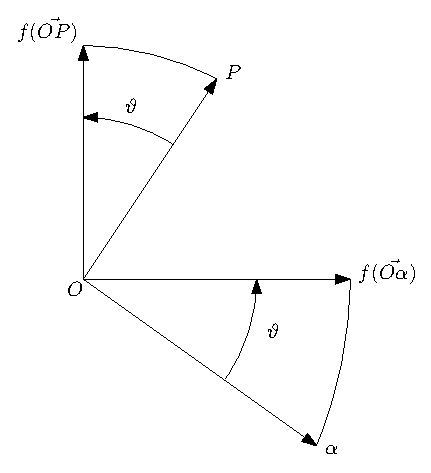
\includegraphics[width=5cm]{img/finiti/imgex4-2-1.eps}
      \caption{$f:V_O^2\to V_O^2$}
    \end{figure}
    Ora, come si vede nel disegno sequente, dati due vettori $\vec{OP}$ e $\vec{OP}^\prime$, sommarli e poi
    ruotare il vettore risultante oppure prima ruotarli e poi sommare i vettori ruotati è equivalente, ovvero
    \clearpage
    \begin{figure}[th]
      \centering
        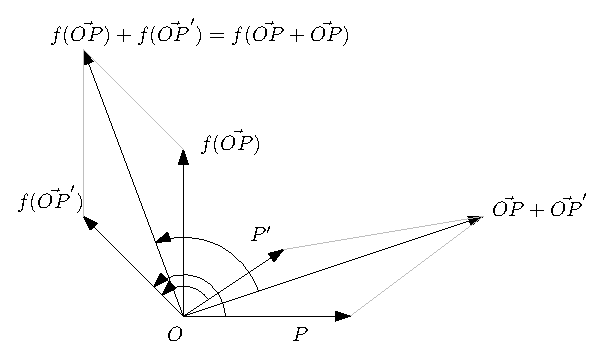
\includegraphics[width=6cm]{img/finiti/imgex4-2-2.eps}
      \caption{$f(\vec{OP})+f(\vec{OP}^\prime)=f(\vec{OP}+\vec{OP})$}
    \end{figure}
    Quindi vale la
    \begin{equation}
      f(\vec{OP})+f(\vec{OP}^\prime)=f(\vec{OP}+\vec{OP})
    \end{equation}
    che ci dice che questa funzione soddisfala proprietà (\ref{applin}) della Definizione \ref{4.1-4.2}\\
    Analogamente, dato un vettore $\vec{OP}$ e un numero reale $c$, moltiplicare il vettore per $c$ e poi
    ruotarlo e poi moltiplicarlo per $c$ è equivalente:
    \begin{figure}[th]
      \centering
        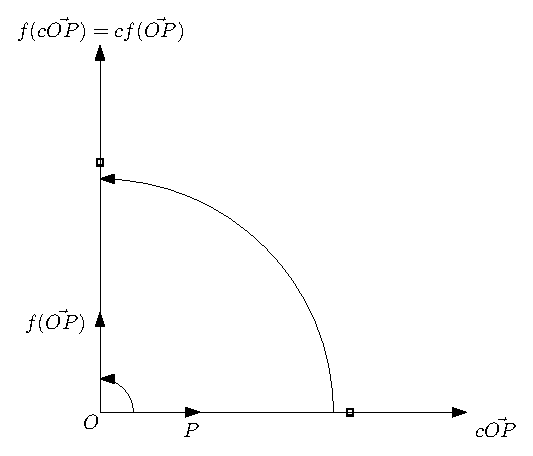
\includegraphics[width=6cm]{img/finiti/imgex4-2-3.eps}
      \caption{$f(c\vec{OP})=cf(\vec{OP})$}
    \end{figure}
    Quindi si ha
    \begin{equation}
      f(c\vec{OP})=cf(\vec{OP})
    \end{equation}
    che ci dice che questa funzione soddisfa anche la proprietà (\ref{matasapplin}), della definizione
    \ref{4.1-4.2} -- Concludiamo quindi che le rotazioni attorno a $O$ sono applicazioni lineari dallo
    spazio vettoriale $V_O^2$ in se stessso.\\
    Possiamo arrivare alla stessa conclusione anche per altre importanti trasformazioni geometriche: ad
    esempio, si consideri la riflessione rispetto a una retta $r$ passante per $O$, che manda ogni vettore
    $\vec{OP}\in V_O^2$ nel vettore simmetrico rispetto alla retta, come nel seguente disegno
    \begin{figure}[th]
      \centering
        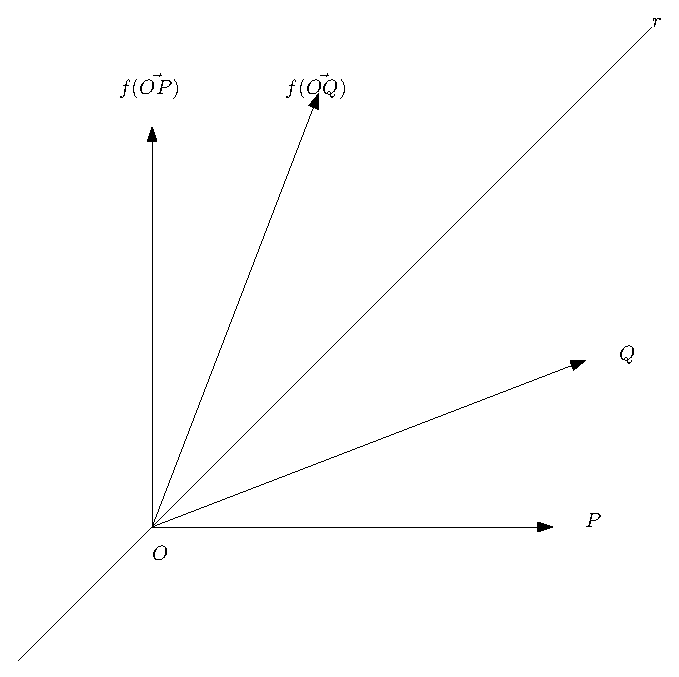
\includegraphics[width=6cm]{img/finiti/imgex4-2-4.eps}
    \end{figure}   
    Allora, come già fatto per le rotazioni, notiamo che, dati due vettori $\vec{OP}$ e $\vec{OP}^\prime$,
    sommarli e poi riflettere il vettore risultante oppure prima rifletterli e poi sommare i vettori riflessi
    è equivalente
    \clearpage
    \begin{figure}[th]
      \centering
        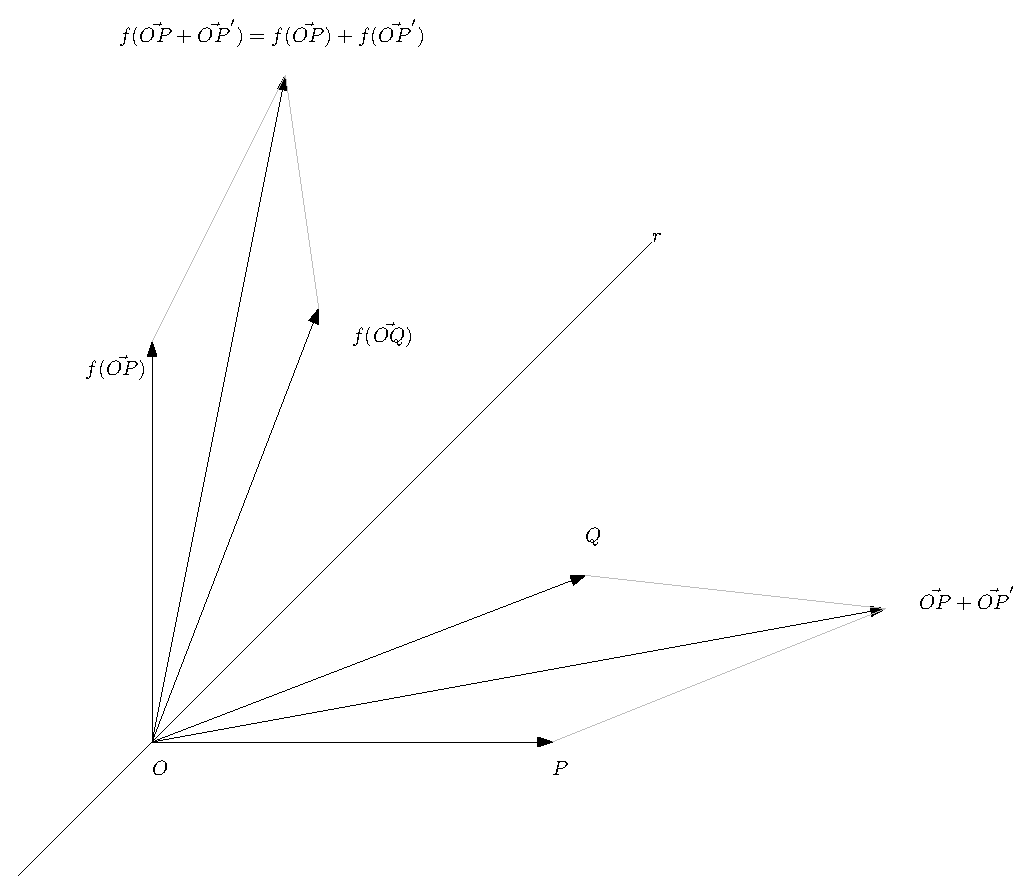
\includegraphics[width=6cm]{img/finiti/imgex4-2-5.eps}
    \end{figure}
    $f\left(\vec{OP}+\vec{OP}^\prime\right)=f\left(\vec{OP}\right)+f\left(\vec{OP}^\prime\right)$ e
    dato uin vettore $\vec{OP}$ e un numero
    reale $c$, moltiplicatore il vettore per $c$ e poi rifletterlo oppure prima rifletterlo e poi moltiplicarlo
    per $c$ è equivalente
    \begin{figure}[th]
      \centering
        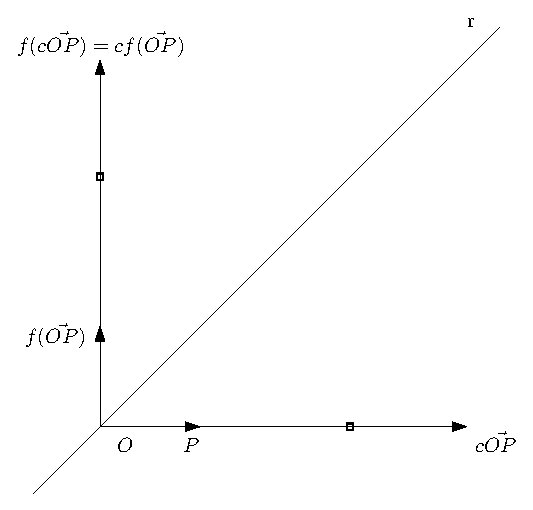
\includegraphics[width=6cm]{img/finiti/imgex4-2-6.eps}
    \end{figure}
      
    $f(c\vec{OP})=cf(\vec{OP})$: quindi concludiamo che anche la riflessione rispetto a una retta ce passa per
    $O$, avendo le proprietà entrambe le proprietà (\ref{4.1-4.2}) richieste nella Definizione (\ref{applin}),
    è un'applicazione lineare $f:V_O^2\to        V_O^2$.\\
    Come terzo esempio esempio di applicazione lineare $V_O^2\to V_O^2$ citiamo la propiezione ortogonale,
    che proieta ortogonalmente i vettori su una retta fissata passante per $O$.
    \begin{figure}[th]
      \centering
        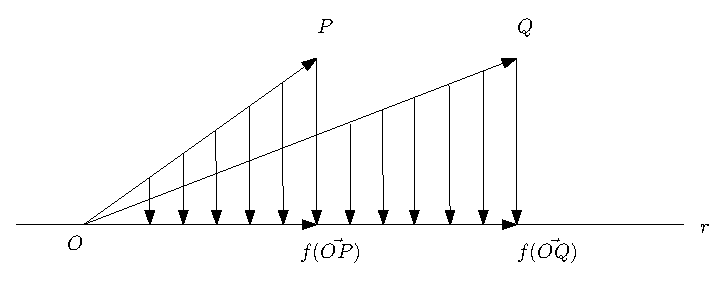
\includegraphics[width=8cm]{img/finiti/imgex4-2-7.eps}
    \end{figure}
      
    per la quale è difficile vedere che valgono ancora le proprieta citate in (\ref{4.1-4.2}).\\
    Analogamente a quanto visto per rotazioni, riflessioni e proiezioni nel piano, anche le corrispondenti
    trasformazioni $V_O^3\to V_O^3$ dello spazio tridimensionale come da proprietà (\ref{4.1-4.2}) della
    Definizione \ref{applin} la rotazione di un angolo fissato $\Theta$ attorno a una retta data passante per $O$
    (detta ase della rotazione)
    \clearpage
    \begin{figure}[th]
      \centering
        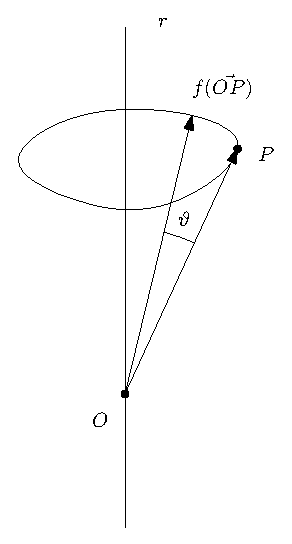
\includegraphics[width=3cm]{img/finiti/imgex4-2-8.eps}
    \end{figure}
    la riflessione rispetto a un piano passante per $O$
    \begin{figure}[th]
      \centering
        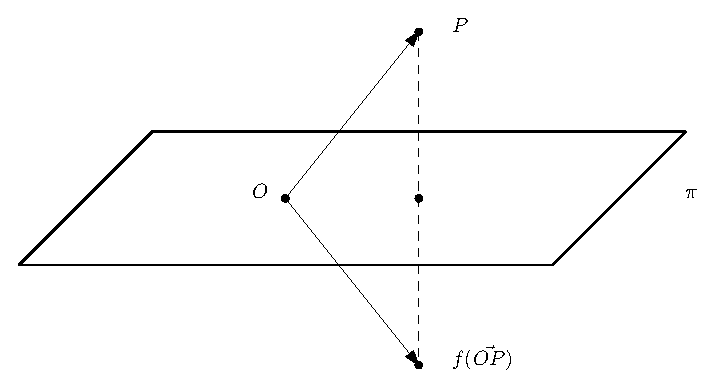
\includegraphics[width=6cm]{img/finiti/imgex4-2-9.eps}
    \end{figure}
      
    e la proiezione ortogonale su un piano passante per l'origine $O$:
    \begin{figure}[th]
      \centering
        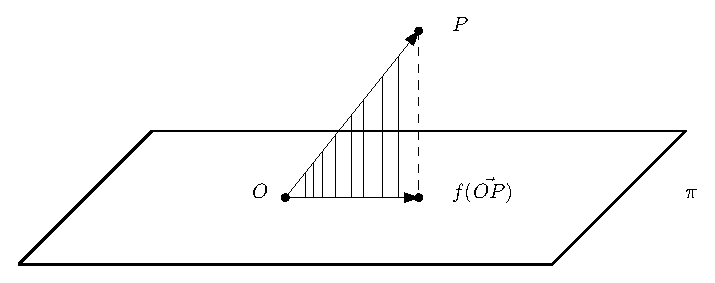
\includegraphics[width=6cm]{img/finiti/imgex4-2-10.eps}
    \end{figure}
    (Quest'ultima può anche essere vista come applicazione $f:V_O^3\to V_O^2$ se vediamo il piano su cui
    proiettiamo come spazio vettoriale a se stante).
  \end{esempio}
\end{definizione}

\section{Matrice associata a un'applicazione lineare}
\label{sec:matassaunapplin}
Una delle caratteristiche fondamentali di un'applicazione lineare $f:V\to W$ è che, se gli spazi $V$ e $W$ hanno
dimensione finita, allora $f$ può essere rappresentata da una matrice.\\ Vediamo i dettagli: sia $f:V\to W$
un'applicazione lineare, e siamo $B_V=\left\{v_1,v_2,\dots,v_n\right\}$ e $B_W=\left\{w_1,w_2,\dots,w_n\right\}$
basi di $V$ e $W$ rispettivamente. Allora, come sappiamo ogni vettore $v\in V$ può essere identificato con una
$n-$upla $\left(x_1,x_2,\dots,x_n\right)$, quella delle sua coordinate rispetto alla base $B_V$ (ovvero
$v=x_1v_1+x_2v_2+\dots+x_nv_n$), e analogamente ogni vettore $w\in W$ può rispetto alla base $B_W$ (ovvero
$w=y_1w_1+y_2w_2+\dots+y_mw_m$). Con questo identificazioni, la $f$ può essere pensata come una funzione
$\mathds{K}^n\to\mathds{K}^m$ che associa a ogni $n$-upla. Ci proponiamo di trovare l'espressione esplicita di
tale funzione. A questo scopo, sia $(x_1,\dots,x_n)$ la $n$-upla delle coordinate di un vettore $v\in V$, ovvero
come abbiamo ricevuto sopra $v=x_1v_1+\dots+x_nv_n$. Allora la sua immagine $f(v)$ sarà
\begin{equation*}
  f(v)=f(x_1v_1+\dots+x_nv_n) =
\end{equation*}
(usando le proprietà un'applicazione lineare)
\begin{equation}
  =f(x_1v_1)+\dots+f(x_nv_n)=x_1f(v_1)+\dots+x_nf(v_n).
\end{equation}
Ora, ciascuno dei vettori $f(v_1),f(v_2),\dots,f(v_n)$ che compare nella ({\bf 4.5}) appartiene al codominio $W$
della funzione, e quindi potrà essere espresso come combinazione lineare dei vettori $w_1,w_2,\dots,w_m$ della
base $B_W$ fissata per $W$:
\clearpage
\begin{equation}
  f(v_1)=a_{11} w_1+a_{21}w_2+\dots+a_{m1}w_m
\end{equation}
\begin{equation*}
  \vdots
\end{equation*}
\begin{equation}
  f(v_1)=a_{1n} w_1+a_{2n}w_2+\dots+a_{mn}w_m
\end{equation}
Ora, sostituendo queste espressioni nella ({\bf 4.5}) si ottiene
\begin{equation*}
  f(v)=x_1(a_{11} w_1+a_{21}w_2+\dots+a_{m1}w_m) +\dots+ x_n(a_{1n} w_1+a_{2n}w_2+\dots+a_{mn}w_m)=
\end{equation*}
(svolgendo i conti e mettendo in evidenza i vettori)
\begin{equation}
  =(a_{11}x_1+\dots+a_{1n}x_n)w_1+\dots+(a_{m1}x_1+\dots+a_{mn}x_n)w_m
\end{equation}
Questa uguaglianza ci sta dicendo che le coordinate del vettore $f(v)$ rispetto alla base $B_W=\left\{w_1,w_2,
  \dots,w_m\right\}$ sono date da $a_{11}x_1+\dots+a_{1n}x_n,\dots,a_{m1}x_1+\dots+a_{mn} x_n$ e quindi che,
tradotta in coordinate, la nostra applicazione lineare può essere identificata con la funzione $\mathds{K}^n\to
\mathds{K}^m$ che associa a ogni $n$-upla $(x_1,\dots,x_n)$ la $m$-upla formata dai coefficienti che appiono nella
({\bf 4.8}), ovvero
\begin{equation}
  \begin{pmatrix}
    x_1\\
    x_2\\
    \vdots\\
    x_n
  \end{pmatrix} \to
  \begin{pmatrix}
    a_{11}x_1+a_{12}x_2+\dots+a_{1n}x_n\\
    a_{21}x_1+a_{22}x_2+\dots+a_{2n}x_n\\
    \vdots\\
    a_{m1}x_1+a_{m2}x_2+\dots+a_{mn}x_n
  \end{pmatrix}
\end{equation}
I coefficienti che compaiono nella ({\bf 4.9}) formano una matrice con $m$ righe e $n$ colonne
\begin{equation*}
  A=
  \begin{pmatrix}
    a_{11} &a_{12}&\dots&a_{1n}\\
    a_{21} & a_{22}&\dots& a_{2n}\\
    \dots\\
    a_{m1} & a_{m2} &\dots&a_{mn}
  \end{pmatrix}
\end{equation*}
che chiamaremo la \textit{matrice associata all'applicazione lineare rispetto alle basi $B_V$ e $B_W$}. In base
alle (\textbf{4.6}), \dots{}, (\textbf{4.7}) tale matrice può essere definita come \textit{la matrice che ha sulle
  colonne le coordinate dei vettori $f(v_1),\dots,f(v_n)$ (ovvero le immagini dei vettori della base $B_V$
  fissata nel dominio) rispetto alla base $B_W$ fissata nel codominio}.\\
Denoteremo $M_{B_wB_V}(f)$ la matrice associata a un'applicazione lineare $f:V\to W$ rispetto alle basi $B_V$ e
$B_W$.\\
Se dominio e codomio dell'applicazione coincidono, ovvero si ha una funzione linerare $f:V\to V$ (tale
applicazione si dicono \textit{endomorfismi}), allora è possibile fissare la stessa base $B_V$ sia nel dominio
che nel codominio, e calcolare la matrice associata $M_{B_wB_V}(f)$. Come vedremo, la matrice associata a
un'applicazione lineare ci dà tutte le informazioni di cui abbiamo bisogno sull'applicazione, e usando gli
strumenti imparati nei capitoli precedenti (\textit{rango, determinante}) saremo in grado di capire molte
proprietà della funzione data. Prima di fare ciò, vediamo subito alcuni esempi di calcolo della matrice
associata.
\begin{esempio}
  \label{es:4.3}
  \begin{enumerate}
  \item Sia $f:V_O^2\to V_O^2$ la rotazione attorno a $O$ di un angolo fissato $\Theta$\footnote{abbiamo visto nel
      nel paragrafo precedente si tratta di un'applicazione lineare}. Per calcolare la matrice associata, fissiamo
    una base $B$ formata da due vettori $=v_1=\vec{OP}_1$ e $v_2=\vec{OP}_2$ dlla stessa lunghezza e
    perpendicolari tra loro, come nel disegno
    \begin{figure}[th]
      \centering
        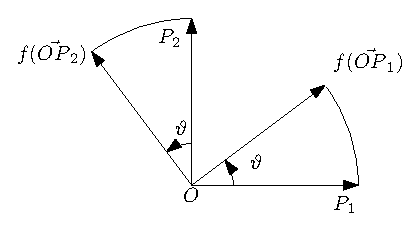
\includegraphics[width=6cm]{img/finiti/imgex4-3-1.eps}
    \end{figure}

    e determiniamo la matrice $M_B(f)$.\\
    A questo scopo, come afferma la difinizione di matrice associata dobbiamo trovare le coordinate di $f(v_1)$ e
    $f(v_2)$ rispetto a $B$, ovvero esprimere $f(\vec{OP}_1)$ e $f(\vec{OP}_2)$ come combinazione lineare
    $x_1\vec{OP}_1+x_2\vec{OP}_2$ dei vetori della base $B$. Iniziamo con $f(\vec{OP}_1)$: come si vede nel
    disegno seguente
    \clearpage
    \begin{figure}[th]
      \centering
        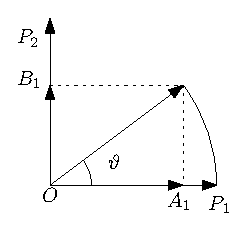
\includegraphics[width=6cm]{img/finiti/imgex4-3-2.eps}
    \end{figure}

    (nel quale stiamo denotando $R_1$ il punto finale del vettore ruotato $f(\vec{OP}_1)$) si ottine
    $f(\vec{OP}_1)=\vec{OP}_1=\vec{OA}_1+\vec{OB}_1$, essendo $A_1$ e $B_1$ le proiezioni ortogonali di $R_1$
    sui vettori di base. Ora, chiaramente $\vec{OA}_1=x_1\vec{OP}_1$ e $\vec{OB}_1=x_2\vec{OP}_2$, dove $x_1$ è
    dato dal rapporto $\frac{\abs{\vec{OA}_1}}{\vec{OP}_1}$ tra la lunghezza di $\vec{OA}_1$ e quella di
    $\vec{OP}_1$, mentre $x_2$ è dato dal rapporto $\frac{\abs{\vec{OB}_1}}{\vec{OP}_2}$ tra la lunghezza di
    $\vec{OB}_1$ e quella di $\vec{OP}_2$. Ma essendo la lunghezza di $\vec{OP}_1$ uguale alla lunghezza di
    $\vec{OR}_1=f(\vec{OP}_1)$\footnote{La rotazione non modifca la lunghezza dei vettore, essi restano
      inveriati anche se cambiano la loro angolazione.} possimo dire che $x_1$ è uguale al rapporto tra la
    lunghezza del cateto $\vec{OA}_1$ e quella dell'ipotenusa $\vec{OP}_1$ del triangolo rettangolo $OR_1A_1$,
    ovvero (esendo il cateto in questione adiacente all'angolo), $x_1=\cos\Theta$. \\
    Analogamente, poiché $\vec{OP}_1$ ha la stessa lunghezza di $\vec{OP}_1$ e quindi di $\vec{OR}_1$, mentre
    $\vec{OB}_1$ ha la stessa lunghezza del segmento $A_1R_1$, si ha 
    \begin{equation*}
      x_2=\frac{\abs{\vec{OB}_1}}{\abs{\vec{OP}_2}}=\frac{\abs{A_1R_1}}{OR_1}
    \end{equation*}
    ovvere\footnote{Essendo il rapporto tra il cateto $A_1R_1$, opposto all'angolo $\Theta$, e l'ipotenusa
      $OR_1$ del triangolo rettangolo $OR_1A_1$}, $x_2=\sin \Theta$. Riassumendo,
    \begin{equation}
      f(\vec{OP}_1)=\vec{OR}_1=\vec{OA}_1+\vec{OB}_1=\cos\Theta \vec{OP}_1+\sin \Theta \vec{OP}_2
    \end{equation}
    Ora, facciamo un ragionamento analogo per determinare $f(\vec{OP}_2)$: come si vede nel disegno seguente
    \begin{figure}[th]
      \centering
        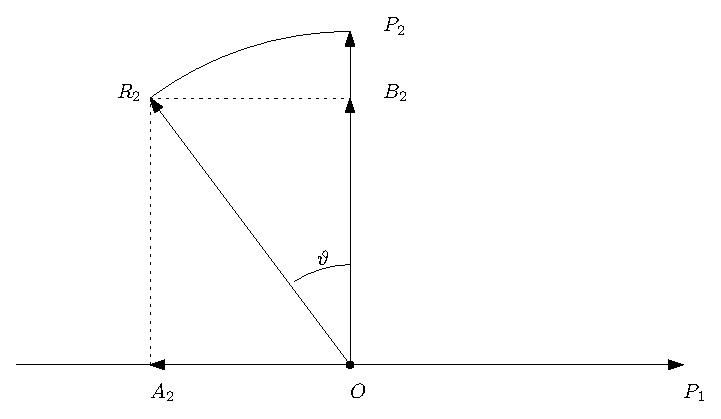
\includegraphics[width=6cm]{img/finiti/imgex4-3-3.eps}
    \end{figure}
      
    (nel quale stiamo denotando $R_2$ il punto finale del vettore ruotato $f(\vec{OPT})$) si ha
    $f(\vec{OP}_2)=\vec{OR}_2=\vec{OA_2}+\vec{OB_2}$. Ora, chiaramente $\vec{OA}_2=-x_1\vec{OP}_1$, dove $x_1$ è
    dato dal rapporto $\frac{\abs{\vec{OA}_2}}{\abs{\vec{OP}_1}}$ tra la lunghezza di $\vec{OA}_2$ e quella di
    $\vec{OP_1}$ (il segno meno è dovuto dal fatto che $\vec{OA}_2$ ha verso opposto rispetto a $\vec{OP}_1$) e
    $\vec{OB}_2=x_2\vec{OP}_2$, dove $x_2$ è dato dal rapporto $\frac{\abs{\vec{OB}_2}}{\abs{\vec{OP}_2}}$ tra la
    lunghezza di $\vec{OB}_2$ e quella di $\vec{OR}_2$. Ma essendo la lunghezza di $\vec{OP}_1$ uguale alla
    lunghezza di $\vec{OP}_1$ uguale alla lunghezza di $\vec{OP}_2$ e quindi di $\vec{OR}_2=f(\vec{OP}_2)$
    (sempre perché la rotazione non modifica la lunghezza dei vettori), mentre, la lunghezza di $\vec{OA}_2$ è
    uguale alla lunghezza del segmento $R_2B_2$, possiamo dire che $x_1$ è uguale al rapporto tra la lunghezza
    del cateto $R_2B_2$ e quella dell'ipotenusa $OR_2$ del triangolo rettangolo $OR_2B_2$, ovvero (essendo il
    cateto in questione opposto all'angolo), $x_2=\cos\Theta$.\\
    Riassumendo,
    \begin{equation}
      f(\vec{OP}_2)=\vec{OR}_2=\vec{OA}_2+\vec{OB_2}=-\sin\Theta\vec{OP}_1+\cos \Theta\vec{OP}_2
    \end{equation}
    \clearpage
    Quindi, (\textbf{4.10}) e (\textbf{4.11}) ci dicono che la matrice associata a $f$ rispetto a $B$ avrà sulla
    prima colonna $(\cos\Theta,\sin\Theta)$\footnote{le coordinate di $f(\vec{OP}_1)$ rispetto a $B$} e sulla
    seconda colonna $(-\sin\Theta,\cos\Theta)$ (le coordinate di $f(\vec{OP})$ rispetto a $B$), ovvero
    \begin{equation}
      M_B(f)=
      \begin{pmatrix}
        \cos\Theta & -\sin \Theta\\
        \sin\Theta & \cos \Theta
      \end{pmatrix}
    \end{equation}
    Come visto nel (\textbf{4.9}), abbiamo allora che la rotazione, in coordinate, si traduce nella funzione
    $f:\mathds{R}^2\to\mathds{R}^2$ data da
    \begin{equation}
      (x_1,x_2)\mapsto (\cos\Theta x_1-\sin\Theta x_2,\sin\Theta x_1+\cos\Theta x_2)
    \end{equation}
    Ad esempio, scegliamo $\Theta=\frac{\pi}{4}$ e sostituiamo in $(4.12)$ e $(4.13)$, ottenendo rispettivamente
    (si ricordi che $\cos\frac{\pi}{4}=\sin\frac{\pi}{4}=\frac{\sqrt{2}}{2}$)
    \begin{equation*}
      M_B(f)=
      \begin{pmatrix}
        \frac{\sqrt{2}}{2} & -\frac{\sqrt{2}}{2} \\
        \frac{\sqrt{2}}{2} & \frac{\sqrt{2}}{2}
      \end{pmatrix}.
    \end{equation*}
    e anche
    \begin{equation}
      (x_1,x_2)\mapsto
      \begin{pmatrix}
        \frac{\sqrt{2}}{2}x_1+\frac{\sqrt{2}}{2}x_2,\frac{\sqrt{2}}{2}x_1+\frac{\sqrt{2}}{2}x_2
      \end{pmatrix}
    \end{equation}
    Per illustrare come questa semplice funzione $\mathds{R}^2\to\mathds{R}^2$ rappresenti effettivamente la
    rotazione di $\frac{\pi}{4}$, prendiamo ad esempio il vettore $v=v_1+v_2$, che come si vede nel disegno
    seguente coincide con la diagonale del quadrato che ha $v_1$ e $v_2$ come lati:
    \begin{figure}[th]
      \centering
        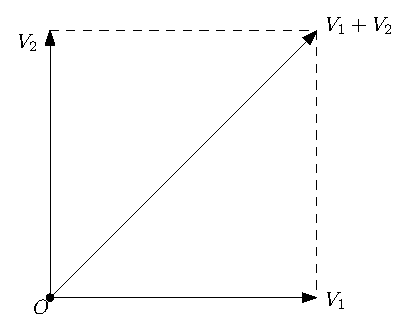
\includegraphics[width=4cm]{img/finiti/imgex4-3-4.eps}
    \end{figure}

    Tale vettore ha quindi come coordinate rispetto a $B$ la coppia $(x_1,x_2)=(1,1)$. In base alla
    \textbf{(4.14)}, le coordinate di $f(v)$ rispetto a $B$ sono date da
    \begin{equation*}
      \frac{\pi}{4}*1-\frac{\pi}{4}*1,\frac{\pi}{4}*1+\frac{\pi}{4}*1=(0,\sqrt{2})
    \end{equation*}
    ovvero deve essere $f(v)=0v_1+\sqrt{2}v_2=\sqrt{2}v_2$.\\
    In effetti, tale risultato ottenuto analicamente in coordinate è confermato dall'analisi grafica, che ci
    dice che il vettore $f(v)$ che si ottiene ruotando la diagonale $v$ del quadrato di $\frac{\pi}{4}$ è proprio
    proporzionale al vettore $v_2$ e la sua lunghezza è proprio $\sqrt{2}$ volte la lunghezza di $v_2$ (in
    quasto $v$ coincideva con la diagonale del quadrato di lati $v_1$ e $v_2$):
    \begin{figure}[th]
      \centering
        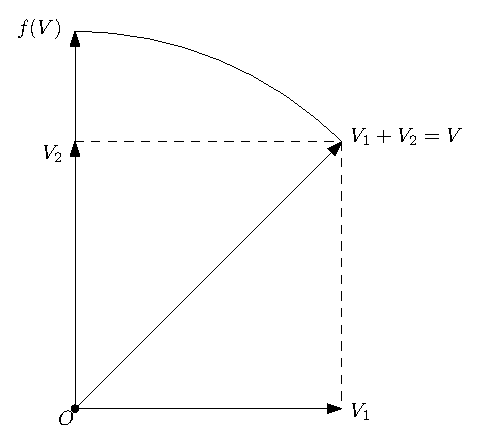
\includegraphics[width=4cm]{img/finiti/imgex4-3-5.eps}
    \end{figure}
  \item Sia $V=V_O^2$ lo spazio vettoriale dei vettori applicati in un punto $O$ nel piano e sia $f:V_o^2\to
    V_O^2$ la proiezione ortogonale su una retta fizzata $r$ passante per $O$\footnote{abbiamo visto nel
      paragrafo precedente che si tratta di un'applicazione lineare}.\\
    Ora, notiamo che quando proiettiamo $v_1$ ortogonalmente su $r$, otteniamo un vettore $v$ che sta sulla retta
    ed è lungo come metà della diagonale del quadrato i cui lati sono $v_1$ e $v_2$: essendo tale diagonale,
    per definizione di somma tra vettori, coincidente con $v_1+v_2$, abbiamo quindi che $f(v_1)=
    \frac{1}{2}(v_1+v_2)=\frac{1}{2}v_1+\frac{1}{2}v_2$; analogamente, come si vede dal disegno, anche
    proiettando $v_2$ sulla retta di ottiene lo stesso vettore $v$, quindi si ha anche $f(v_2)=
    \frac{1}{2}(v_1+v_2)=\frac{1}{2}v_1+\frac{1}{2}v_2$.
    \begin{figure}[th]
      \centering
        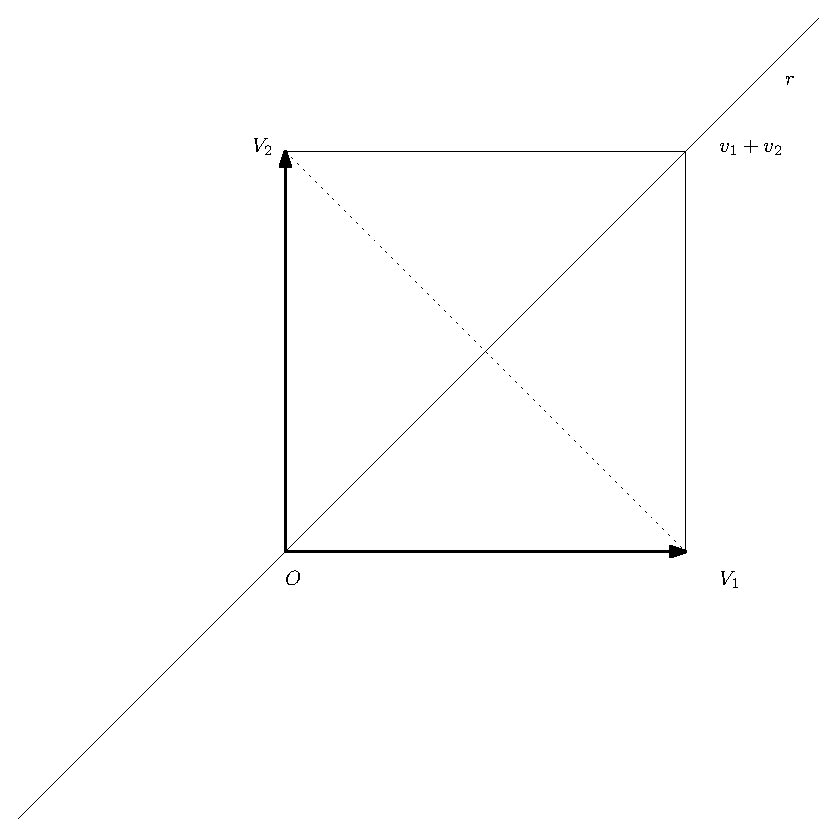
\includegraphics[width=4cm]{img/finiti/imgex4-3-6.eps}
    \end{figure}
    Si vede quindi che le coordinate di $f(v_1)$ rispetto a $B$ sono $\left(\frac{1}{2},\frac{1}{2}\right)$, e
    anche le coordnate di $f(v_2)$ rispetto a $B$ sono $\left(\frac{1}{2},\frac{1}{2}\right)$: disponendo tali
    coordinate rispettivamente sulla prima e sulla seconda colonna, come previsto dalla difinizione di matrice
    associata, si ottiene
    \begin{equation*}
      M_B(f)=
      \begin{pmatrix}
        \frac{1}{2}&\frac{1}{2}\\
        \frac{1}{2} & \frac{1}{2}
      \end{pmatrix}
    \end{equation*}
    e la funzione $\mathds{R^2}\to \mathds{R}^2$ corrispondente
    \begin{equation}
      (x_1,x_2)\mapsto
      \begin{pmatrix}
        \frac{1}{2}x_1+\frac{1}{2}x_2, \frac{1}{2}x_1+\frac{1}{2}x_2
      \end{pmatrix}
    \end{equation}
    ci dà una rappresentazione in coordinarte della proiezione.\\
    Ad esempio, il vettore $v=-v_1+v_2$, che ha coordinate $(-1,1)$ rispetto a $B$, viene mandata in base alla
    \textbf{(4.15)} nel vettore di coordinate
    \begin{equation*}
      \begin{bmatrix}
        \frac{1}{2}(-1)+\frac{1}{2}1, \frac{1}{2}(-1)+\frac{1}{2}1
      \end{bmatrix}=(0,0)
    \end{equation*}
    ovvero nel vettore nullo $\vec{OO}$. Infatti, come si vede dal seguente disegno, tale vettore appartiene
    alla retta passante per $O$ e ortogonale a $r$, e i vettori che giacciono su questa retta vengono chiaramnte
    proiettati sul vettore nullo $\vec{OO}$.
    \begin{figure}[th]
      \centering
        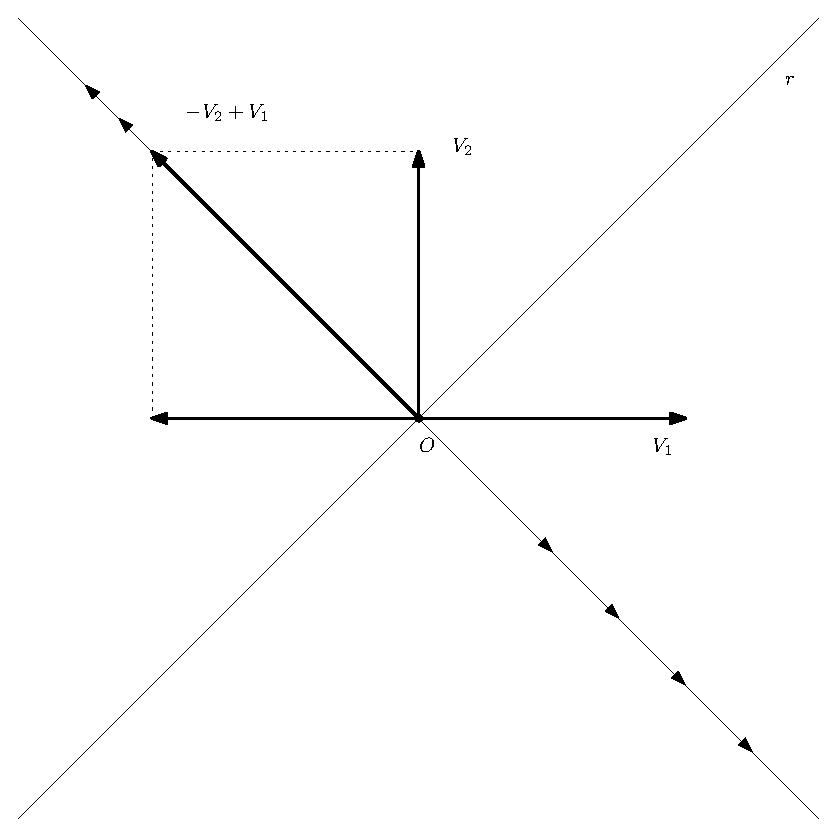
\includegraphics[width=6cm]{img/finiti/imgex4-3-7.eps}
    \end{figure}   
  \item Come ultimo esempio, prendiamo come funzione $f:V_O^2\to V_O^2$ la riflessione rispetto a una retta
    fissata $r$ passante per $O$, ovvero l'endomorfismo che associa a ogni vettore $\vec{OP}$ il suo simmetrico
    rispetto a $r$\footnote{Sappiamo dal primo paragrafo che si tratta di un'applicazione lineare}. Per calcolane
    la matrice associata $M_B(f)$, consideriamo la stessa base $B=\left\{v_1,v_2\right\}$ usata nell'esempio
    precedente.
    \clearpage
    \begin{figure}[th]
      \centering
        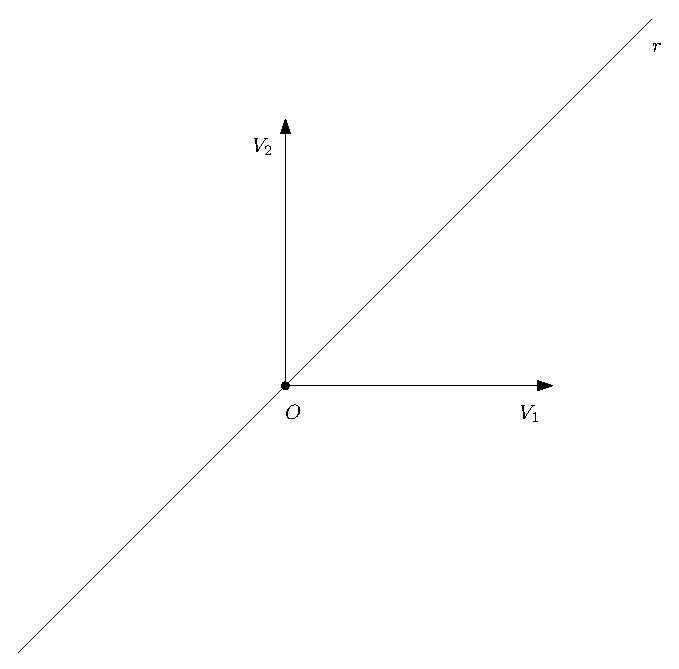
\includegraphics[width=4cm]{img/finiti/imgex4-3-8.eps}
    \end{figure}
    e notiamo che quando riflettiamo $v_1$ rispetto a $r$ otteniamo $v_2$, ovvero $f(v_1)=v_2$, analogamente
    quando riflettiamo $v_2$ rispetto a $r$, otteniamo $v_1$ ovvero $f(v_2)=v_1$.\\
    Quindi, riscrivendo $f(v_1)=v_2$ come $f(v_1)=0v_1+1v_2$ vediamo che le coordinate di $f(v_1)$ rispetto a $B$
    sono $(0,1)$, e analogamente riscrivendo $f(v_2)=v_1$ come $f(v_1)=1v_1+0v_2$ vediamo che le
    coordinate di $f(v_2)$ rispetto a $B$ sono $(1,0)$: disponendo tale coordinate in colonna,
    come previsto dalla definizione della matrice associata, si ottiene
    \begin{equation*}
      M_B(f)=
      \begin{pmatrix}
        0 & 1\\
        1 & 0
      \end{pmatrix}
    \end{equation*}
    Se dato sempre lo stesso endomorfismo, consideriamo invece la base $B^\prime= \{v_1^\prime,
    v^\prime_2$ come nel disegno seguente
    \begin{figure}[th]
      \centering
        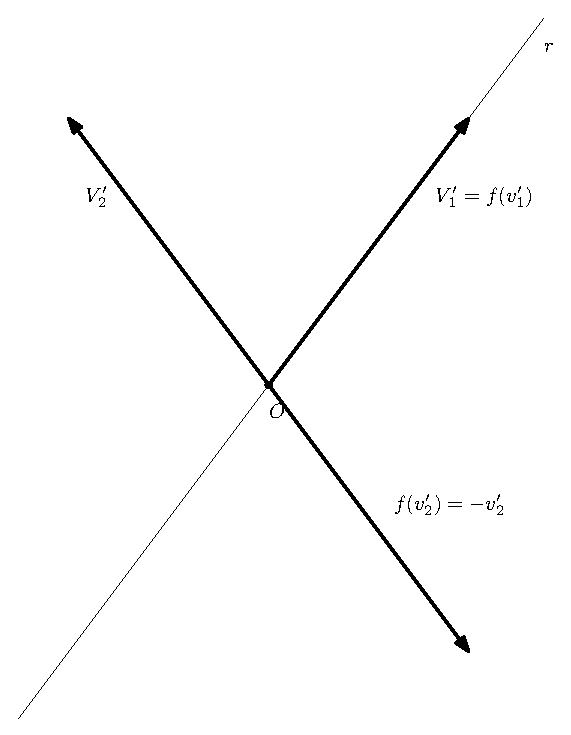
\includegraphics[width=4cm]{img/finiti/imgex4-3-9.eps}
    \end{figure}
    allora si ha che $f(v_1^\prime)=v_1^\prime$ (il vettore $v_1^\prime$ sta sulla retta e quindi
    la riflessione rispetto alla retta lo lascia invariato) e $f(v^\prime_2)=-v^\prime_2$ (il
    vettore $v_2^\prime$ è perpen dicolare alla fetta quindi riflettendolo esso cambia verso),
    cioè $f(v_1^\prime)=1v^\prime_1+0v^\prime_2$ e $f(v_2)=0v_1^\prime+(-1)v_2^\prime$ e quindi
     \begin{equation*}
      M_{B^\prime}(f)=
      \begin{pmatrix}
        1 & 0\\
        0 & -1
      \end{pmatrix}
    \end{equation*}
    Questo esempio illustra il fatto, ovvio che la matrice associata dipenda dalla scelta delle
    basi.
  \end{enumerate}
\end{esempio}

\section{Iniettività e suriettività delle applicazioni lineari}
\label{sec:inie_surie_app_lin}
Il primo problema che affronteremo sulla applicazioni lineari è determinare quando una tale
funzione è iniettiva, suriettiva o biiettiva.

\subsection{Richiami generali}
\label{sec:inie_surie_app_lin_ric_gen}
Ricordiamo che una funzione $f:A\to B$ tra due insiemi $A$ e $B$ si dice \textit{suriettiva} se
ogni elemento del codominio $B$ risulta essere immagine di qualche elemento di $A$ (ovvero, se
per ogni $b\in B$ esiste un $a\in A$ tale che $f(a)=b$).\\
Ad esempio, delle funzioni rappresentate nel seguente disegno, la prima non è
suriettiva\footnote{L'elemento $c\in B$ non è immagine di nessun elemento di $A$},
mentre, la seconda si.
\begin{figure}[th]
  \centering
  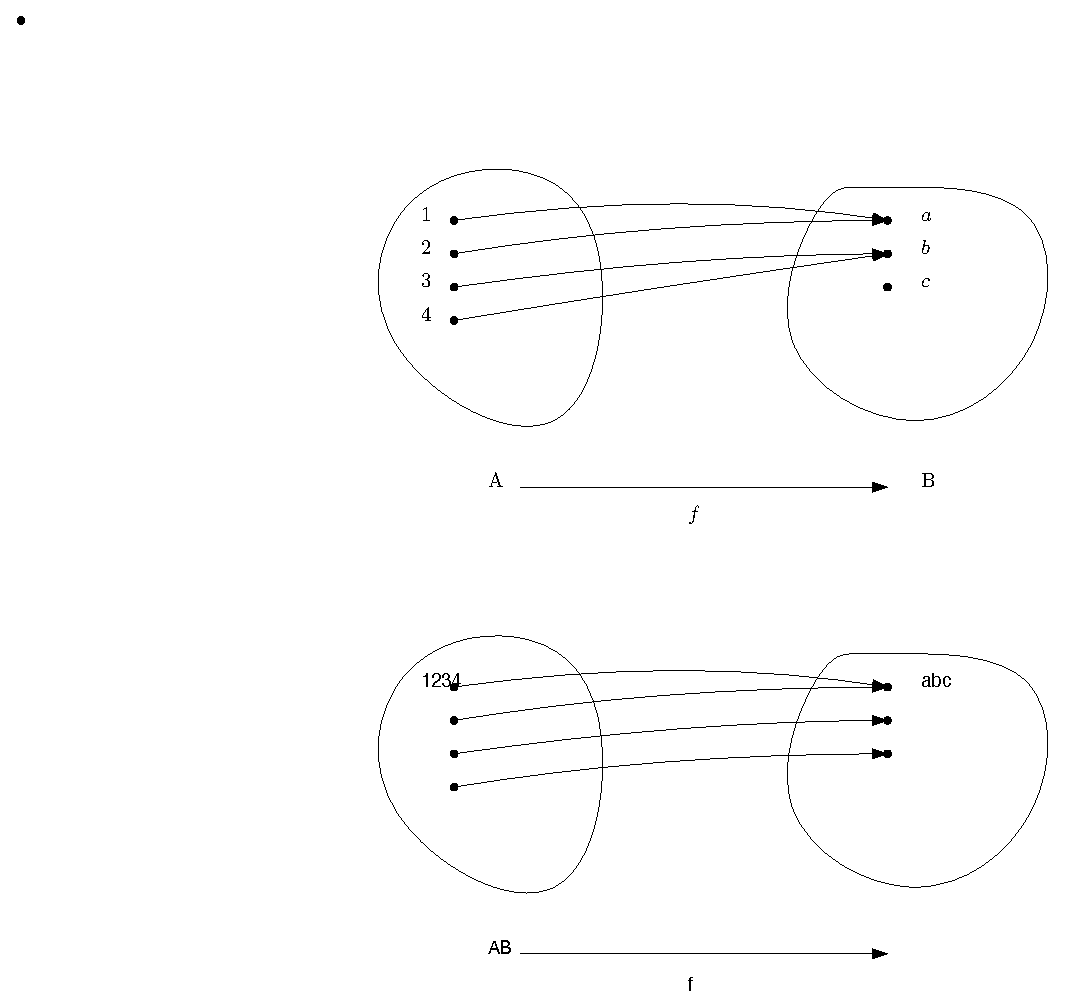
\includegraphics[width=8cm]{img/finiti/imgex4-4-1.eps}
  \caption{differenza tra iniettivo e suriettivo}
\end{figure}
Un modo alternativo di dire che una funzione èsuriettiva è fare riferimento alla cosidetta 
\textit{immagine} $I_m(f)$ di f: per definizione, l'immagine di una funzione $f:A\to B$ è il
sottoinsieme di $B$ costituito da futti gli elementi che sono immagine di qualche elemento di $A$
(in riferimento ai disegni, quegli elementi ``raggiunti da una freccia che provviene da A''),
ovvero
\begin{equation*}
  I_m(f)=\{b\in B | b=f(a) \text{ per qualche } a \in A\}
\end{equation*}
Ad esempio, la funzione sopra nel disegno precedente ha $I_m(f)=\{a,b\}$, mentre la funzione
sotto ha $I_m(f)=\{a,b,c\}$ç una funzione è suriettiva esattamente quando $I_m(f)=B$, ovvero
l'immagine coincide con tutto il codominio\footnote{Dire $I_m(f)=B$ significa in effetti dire
  che ogni elemento di $B$ è immagine di quelche elemento di $A$}.
\begin{figure}[th]
  \centering
  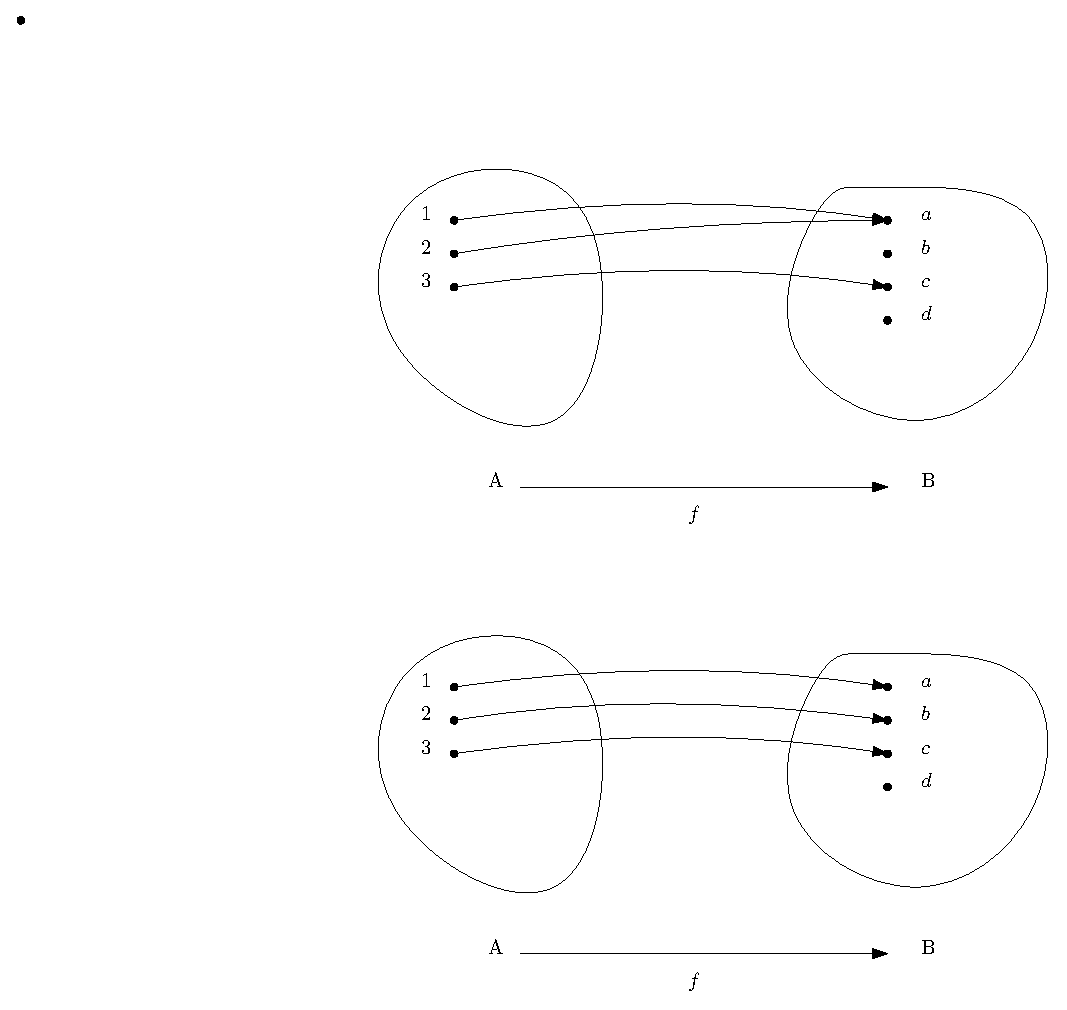
\includegraphics[width=8cm]{img/finiti/imgex4-4-2.eps}
\end{figure}

La nozione di iniettività può essere riformata tramite il concetto di \textit{controimmagine}:
dato un elemento $b$ del codomiono $B$, la sua controimmagine, denotata $f^{-1}(b)$, è l'insieme
di tutti gli elementi di $A$ che hanno $b$ come immagine, ovvero
\begin{equation*}
  f^{-1}(b)=\{a\in A|f(a)=b\}
\end{equation*}
Dal momento che una funzione è iniettiva quando non esistono dhe elementi diversi che hanno la
stessa immagine, dire che una funzione è iniettiva quivale a dire che tutte le controimmagini
che non siano vuote\footnote{se la funzione non è suriettiva, ci saranno elementi $b\in B$ tali
  che non esiste nessun $a\in A$ con $f(a)=b$ e quindi la cui controimmagine $f^{-1}(b)$ non ha
  elementi.} hanno un solo elemento.\\
Ad esempio, per la funzione sofra nel disegno precedente si ha $f^{-1}(a)=\{1,2\},f^{-1}(b)=
\not{0},f^{-1}(c)=\{3\}$: essa non è iniettiva in quanto la controimmagine di a ha due elementi.\\
Per la funzione sotto, invece, si ha $f^{-1}(a)=\{1\}, f^{-1}(b)=\{2\},f^{-1}(c)=\{3\},
f^{-1}(d)=\not{0}$: essa è iniettiva in quanto le controimmagini non vuote hanno tutte un solo
elemento.\\
Infine, una funzione si dice \textit{biiettiva} se è sia inittiva che suriettiva. Ad esempio,
la funzione rappresentata nel sequente disegno è biiettiva.
\begin{figure}[th]
  \centering
  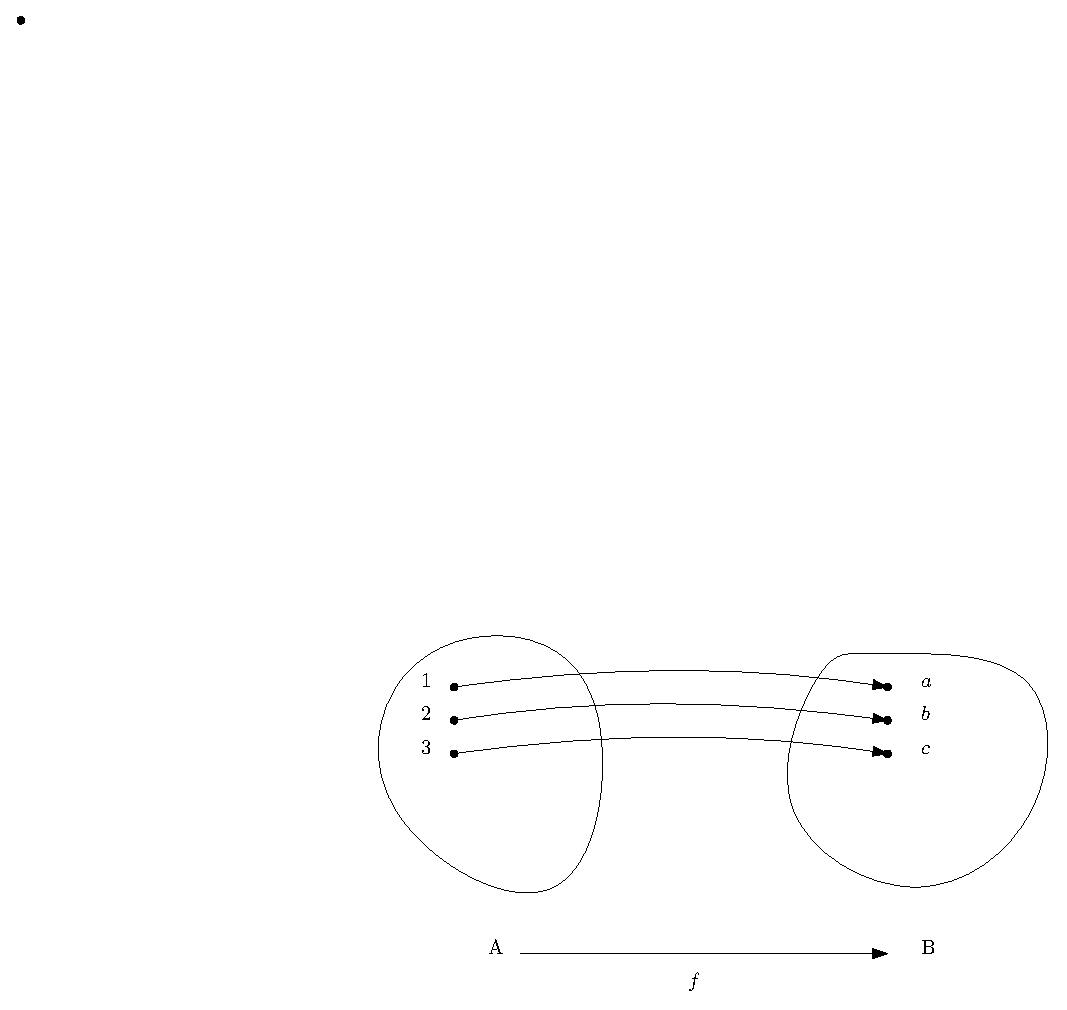
\includegraphics[width=8cm]{img/finiti/imgex4-4-3.eps}
\end{figure}

\subsection{Suriettività delle applicazione lineari}
Abbiamo detto che una funzione $f: A\to B$ è suriettiva se e solo se per ogni elemento di
$b\in B$ esiste un $a\in A$ tale che $f(a)=b$, ovvero equivalentemente se e solo se la sua
immagine $I_m(f)$ coincide con tutto il codominio.\\
Nel caso di un'applicazione lineare $f:V\to W$, vale la seguente importante
\begin{proposizione}
  Sia $f: V\to W$ un'applicazione lineare. Allora $I_m(f)$ è un sottospazio vettoriale di W.
\end{proposizione}
\begin{proof}
  Dobbiamo verificare che $I_m(f)$ è chiuso rispetto alla somma e al prodotto per scalari. Per la
  prima proprietà dobbiamo prendere $w,w^\prime\in I_m(f)$ e vedere se $w+w^\prime\in I_m(f)$. Ora,
  se $w,w^\prime\in I_m(f)$, per definizione di $I_m(f)$ significa che esistono un vettore
  $v\in V$ tale che $w=f(v)$ e un vettore $v^\prime\in V$ tale che $w^\prime=f(v^\prime)$ e un
  vettore $v^\prime\in V$ tale che $w=f(v)$ e un vettore $v^\prime \in V$ tale che
  $w^\prime\in f(v^\prime)$. Ma allora, sfruttando il fatto che $f$ è lineare, si ha
  \begin{equation*}
    w+w^\prime=f(v)+f(v^\prime)=f(v*v^\prime)
  \end{equation*}
  che ci dice che anche $w+w^\prime$ è immagine di un elemento del dominio (cioè $v+v^\prime$) e
  quindi $w+w^\prime\in m(f)$.\\
  Per la chiusura rispetto al prodotto per scalari, dobbiamo verificare che se $w\in I_m(f)$ e
  $c\in\mathds{K}$, allora $cw\in I_m(f)$. Ma, come prima, se $w\in I_m(f)$ allora per
  definizione di $I_m(f)$ esiste un vettore $v\in V$ tale che $w=f(v)$, e quindi, usando sempre
  il fatto che $f$ è linerare,
  \begin{equation*}
    cw=cf(v)=f(cv)
  \end{equation*}
  che ci dice che anche $cw$ è immagine di un elemento del dominio (cioè $cv$) e quindi $cw\in I_m(f)$.
\end{proof}
Il fatto che $I_m(f)$ sia un sottospazio vettoriale ci dice che per determinarla possiamo trovarne un sistema di
generatori o una base. Questo si fa facilmente grazie alla seguente
\begin{proposizione}
  Sia $f:V\to W$ un'applicazione lineare e siamo $v_1,\dots,v_n$ generatori $V$.
  Allora le immagini $f(v_1),\dots,f(v_n)$ generano $I_m(f)$ (in simboli, $I_m(f)=[f(v_1),\dots,f(v_n)]$)
\end{proposizione}
\begin{proof}
  Per definizione di generatori, dobbiamo verificare che ogni vettori $w\in I_m(f)$ si può scrivere come
  combinazione lineare dei vettori $f(v_1),\dots,f(v_n)$. Ora, sappiamo che un vettore $w\in I_m(f)$ è tale che
  $w\in f(v)$ per qualche $v\in V$. Ma essendo per ipotesi $v_1,\dots,v_n$ generatori di $V$, il vettore
  $v$ potrà essere scrittocome loro combinazione lineare $v=x_1v_1+\dots+x_nv_n$. Quindi, sfruttando la
  linearità di $f$ si ha
  \begin{equation*}
    w=f(v)=f(x_1v_1+\dots+x_nv_n)=x_1f(v_1)+\dots+x_nf(v_n)
  \end{equation*}
  che dimostra prprio che $w$ si scrive come combinazione lineare di $f(v_1),\dots,f(v_n)$, come volevamo.
\end{proof}
A questo punto, per determinare se un'applicazione lineare $f:V\to W$ è suriettiva, basta scegliere dei
generatori $v_1,\dots,v_n$ di $V$, prendere le loro immagini $f(v_1),\dots,f(v_n)$ che, come abbiamo appena
visto, formano un insieme di generatori di $I_m(f)$, e poi estrarre da quest'ultimo insieme una base eliminando
gli eventuali vettori che sono dipendenti dai rimanenti: contando i vettori della base ottenuta, sapremo la
dimensione di $I_m(f)$ e quindi $f$ sarà suriettiva se e solo se\footnote{Questa affermazione è giustificato
  dal fatto, che non abbiamo dimostrato, che se $S$ è un sottospazio vettoriale di una spazio vettoriale $V$,
  allora $dim (S)\leq dim (V)$ e le dimensioni coincidono se e solo se $S=V$.} $dim(I_m(f))=dim(W)$.\\
Vediamo come tale criterio di suriettività si rivela particolarmente utile e di semplice applicazione nel caso
dell'applicazioni lineare $L_A:\mathds{K}^n\to \mathds{K}^m$ determinata da una matrice $A$, ovvero della forma
data dalla (4.9)\footnote{Come sappiamo, ogni applicazione lineare puo`essere identificata con una tale
  funzione grazie alla matrice associata}.\\
Ora, se come generatori del dominio $V=\mathds{K}^n$ scegliamo i vettori della base canonica
$v_1=(1.0.\dots,0),v_2=(0,1,\dots,0),v_n=(0,0,\dots,1)$, dalla (4.9) si ha
\begin{equation*}
  f(v_1)=L_A
  \begin{pmatrix}
    1 \\
    0 \\
    \vdots\\
    0
  \end{pmatrix}=
  \begin{pmatrix}
    a_{11}\\
    a_{12}\\
    \vdots\\
    a_{m1}
  \end{pmatrix},
  f(v_2)= L_A
   \begin{pmatrix}
    0 \\
    1 \\
    \vdots\\
    0
   \end{pmatrix}=
   \begin{pmatrix}
    a_{12}\\
    a_{22}\\
    \vdots\\
    a_{m2}
   \end{pmatrix}, \dots, f(v_n)=
   L_A
   \begin{pmatrix}
    0\\
    0\\
    \vdots\\
    1
   \end{pmatrix}=
   \begin{pmatrix}
    a_{1n}\\
    a_{2n}\\
    \vdots\\
    a_{mn}    
   \end{pmatrix}
\end{equation*}
cioè $f(v_1),f(v_2),\dots,f(v_n)$ sono le colonne $C_1,C_2,\dots,C_n$ della matrice $A$ che determina
l'applicazione. Quindi, in base alla Proposizione \textbf{2}, si ha $I_m(f)=\{C_1,c_2,\dots,C_n\}$ e la funzione
è suriettiva se e solo se $dim\{C_1,C_2,\dots,C_n\}=dim(\mathds{K}^m)=m$. Ma poiché la dimensione del sottospazio
generato dalle colonne di una metrice è per definizione il suo rango, concludiamo che \textit{un'applicazione
  del tipo (4.9) è suriettiva se e solo se il rango di $A$ è uguale a $m$}.

\subsection{Iniettività di applicazioni lineari}
Mentre nel caso della suriettività abbiamo visto che per verificare se una funzione $f$ è suriettiva basta
controllare un solo sottoinsieme del codomonio (l'immagine $I_m(f)$), in generale per verificare se $f$ è
iniettiva dobbiamo a priori controllare tutte le controimmagini degli elementi del codominio e verificare che
queste, quando non sono vuote, hanno un solo elemento.\\
Ora, per una generica funzione $f:A\to B$ le controimmagini degli elementi di $B$ sono sottoinsiemi del tutto
indipendenti tra loro: come nel seguente disegno
\begin{figure}[th]
  \centering
  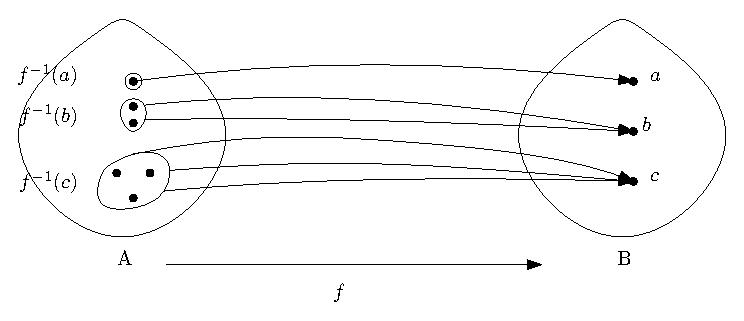
\includegraphics[width=8cm]{img/finiti/imgex4-4-4.eps}
\end{figure}

può accadere che un elemento abbia controimmagine costituine costituita da un solo elemento ma altri abbiamo
controimmagine costituita da più elementi. Vedremo ora invece che le applicazioni lineari hanno il particolare
comportamento per cui le controimmagini degli elementi di $B$, se non sono vuote, o sono \textit{tutte}
costituite da un solo elemento (nel quel caso la funzione non è iniettiva): quindi basta controllare una sola
controimmagine non vuota per capire come sono fatte tutte le altre. Più precisamente abbiamo la seguente
\begin{proposizione}
  Sia $f: V\to W$ un'applicazione lineare. Allora valgono i seguenti fatti:
  \begin{description}
  \item[(i)] la controimmagine $f^{-1}(\bar{0})=\{v\in V | f(v)=\bar{0}\}$ del vettore nullo di $W$ è un
    sottomatrice vettoriale di $V$ (detto \textit{nucleo di} $f$ denotato $N(f)$)
  \item[(ii)] per ogni $w_0\in W$, la controimmagine $f^{-1}(w_0)$ di $w_0$,  non è vuota, è un sottospazio
    affine di $V$, e più precisamente
    \begin{equation*}
      f^{-1}(w_0)=v_0+N(f)=\{v_0+n|n\in N(f)\}
    \end{equation*}
    dove $v_0$ è un qualunque elemento fissato d $f^{-1}(w_0)$.
  \end{description}
\end{proposizione}
\begin{proof}
  Per dimostrare $(i)$, iniziamo con l'osservare che il nucleo di $f$ non è mai vuoto, in quanto il vettore
  nullo di $V$ (che, con un abuso di notazione, denotiamo ancora $\bar{0}$) è sicuramente tale che
  $f(\bar{0})=\bar{0}$: infatti, possiamo il vettore nullo $\bar{0}$ di $V$ come $0v$ (dove $v$ è un qualunque
  vettore di $V$) e quindi, sfruttando la linearità di $f$, si ha $f(\bar{0})=f(0v)=0f(v)=\bar{0}$.\\
  Siano $v,v^\prime$ due vettori di $N(f)$, cioè $f(v)=\bar{0}$. Allora, essendo $f$ lineare,
  \begin{eqnarray*}
    f(v+v^\prime)=f(v)+f(v^\prime)=\bar{0}+\bar{0}=\bar{0}
  \end{eqnarray*}
  e quindi anche $v+v^\prime\in N(f)$: questo ci dice che $N(f)$ è chiuso rispetto alla somma.
  Dati invece un vettore $v$ del nucleo\footnote{quindi $f(v)=\bar{0}$} e uno scalare $c\in
  \mathds{K}$, allora, sempre per la linearità di $f$,
  \begin{eqnarray*}
    f(cv)=cf(v)=c\bar{0}=\bar{0}
  \end{eqnarray*}
  ovvero $cv\in N(f)$: questo ci dice che $N(f)$ chiuso rispetto al prodotto per scalari -- La
  \textit{(i)} è dimostrata.\\
  Per dimostrare la \textit{(ii)}, ovvero l'ugualianza $v=N(f)=f^{-1}(w_0)$, dobbiamo dimostrare
  che ogni elemento di $v_0+N(f)$ sta nella controimmagine $f^{-1}(w_0)$ appartiene a $v_0+N(f)$
  (ovvero l'inclusione opposta $f^{-1}(w_0)$). Per dimostrare la prima inclusione, consideriamo il
  generico elemento di $v_0=N(f)$, cioè, per definizione di sottospazio affine, un vettore $v$ del
  tipo $v=v_0+n$, con $n\in N(f)$. Allora
  \begin{equation*}
    f(v)=f(v_0+n)=f(v_0)+f(n)=f(v_0)=\bar{0}=f(v_0)=w_0
  \end{equation*}
  (nella seconda uguaglianza abbiamo usato il fatto che $f$ è lineare, nella terza il fatto che $n$ appartiene
  al nucleo di $f$ e quindi $f(n)=\bar{0}$). Abbiamo dimostrato che $f(v)=w_0$, cioè $v$ appartiene alla
  controimmagine $f^{-1}(w_0)$ di $w_0$, come volevamo.\\
  Per dimostrare la seconda inclusione, consideriamo un qualunque elemento $v$ della controimmagine di $w_0$,
  cioè $f(v)=w_0$. Essendo $w_0=f(v_0)$, si ha quindi $f(v)=f(v_0)$, da cui, portando a primo membro,
  $f(v)-f(v_0)=\bar{0}$. Essendo $f$ lineare, quest'ultima uguaglianza può essere riscritta $f(v-v_0)=\bar{0}$,
  il che ci dice che il vettore $v-v_0$ appartiene al nucleo $N(f)$ di $f$. Ma allora, osservando che chiaramente
  $v=v_0+(v-v_0)$, vediamo che $v$ si decompone proprio come somma di $v_0$ e di un elemento del nucleo $N(f)$,
  $v\in v_0+N(f)$, come volevamo.
\end{proof}
La proposizione appena dimostrata afferma in pratica che tutte le controimmagini non vuote
di un'applicazione lineari $f$ sono ``copie'' o traslati del nucleo $N(f)$: per illustrare ciò,
consideriamo ad esempio lo spazio $V_0^2$ dei vettori nel piano applicati in = e l'applicazione
lineare $f:V^2_O \to V^2_O$ data dalla proiezione ortogonale su una retta $r$ fissata.\\
Come si vede, un vettore viene proiettato sul vettore nullo $\vec{OO}$ (cioè appartiene al
nucleo $N(f)$ della funzione) se e solo se appartiene alla retta passante per $O$ e ortogonale
a $r$, come i vettori $\vec{OP}. \vec{OQ}$ del disegno sequente
\begin{figure}[th]
  \centering
  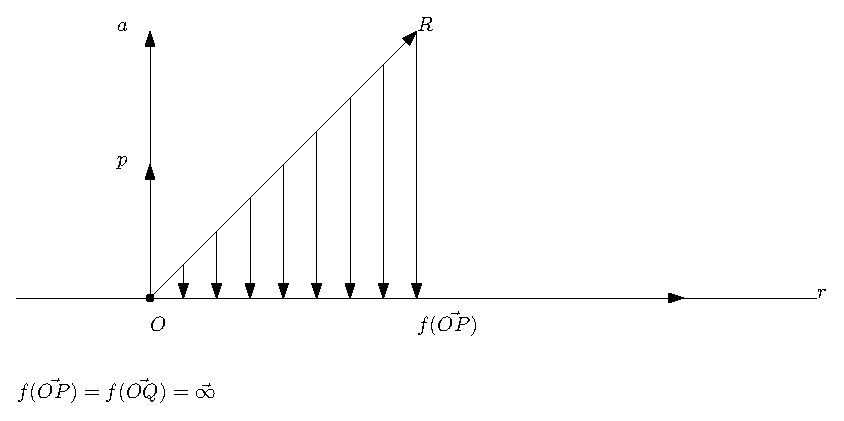
\includegraphics[width=8cm]{img/finiti/imgex4-4-5.eps}
\end{figure}

Ma, come sappiamo, i vettori che stanno su una retta per $O$ formano un sottospazio vettoriale:
questo conferma che il nucleo N(f) è un sottospazio vettoriale.
Per verificare ora che le contro immagini non vuote sono copie traslati del nucleo, consideriamo
come nel disegno seguente
\begin{figure}[th]
  \centering
  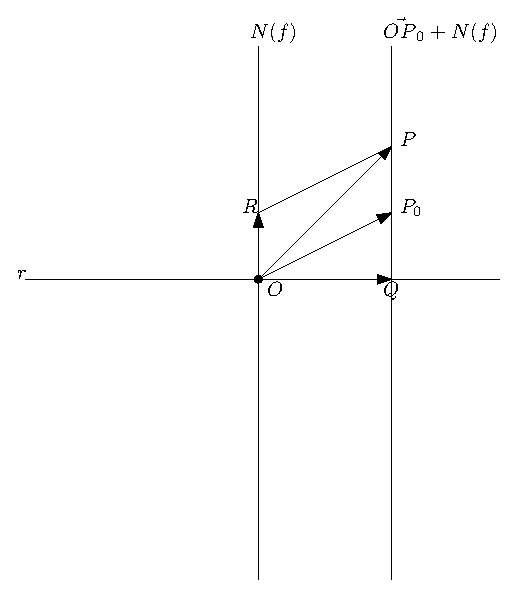
\includegraphics[width=5cm]{img/finiti/imgex4-4-6.eps}
\end{figure}

Un qualunque vettore $\vec{OP}$ che stia nell'immagine di $f$, diciamo $\vec{OQ}=f(\vec{OP}_0)$:
la sua controimmagine, oltre che da $\vec{OP}_0$, è data da tutti i vettori $\vec{OP}$ che
vengono proiettati su $\vec{OQ}$, cioè, come si vede nel disegno, tutti i vettori che hanno
secondo estremo sulla retta ortogonale a $r$ e passante per $Q$.
\clearpage
Ognuno di tali vettori $\vec{OP}$ si decompone copme somma di $\vec{OP}_0$ più un vettore
$\vec{OR}$ appartenente al nucleo $N(f)$: quindi, come previsto dalla Proposizione <++>, la
controimmagine $f^{-1}(\vec{OQ})$ è dato dal sottospazio affine $\vec{OP}_0+N(f)$, traslato
della ortogonale a $r$ e passante per $O$ che rappresenta il nucleo.\\
La Proposizione <++> ha come immediato corollario il seguente criterio necessario e sufficiente di iniettivi per
un'applicazione lineare:
\begin{corollario}
  Un'applicazione lineare $f:V\to W$ è iniettiva se e solo se $N(f)=\{\bar{0}\}$. 
\end{corollario}
\begin{proof}
  Un'applicazione lineare è iniettiva se e solo se la controimmagine di ongi elemento $w_0\in W$, se non è
  vuota\footnote{Cosa che succede se $w_0$ non st nell'immagine dell'applicazione}, contiene un solo elemento.
  Ma poiché, come abbiamo visto nella proposizione, la controimmagine di ogni elemento $w_0$ dell'immagine è del
  tipo $v_0+N(f)$, allora questa conterrà un solo elemento $v_0$ esattamente quando il nucleo contiene il solo
  vettore nullo $\bar{0}$m cioè $N(f)=\{\bar{0}\}$.
\end{proof}
Notiamo che il fatto che il nucleo sia un sottospazio vettoriale ci ditce che possiamo parlare di base e
dimensione del nucleo, e che possiamo riformulare il criterio di inietività per un'applicazione lineare $f$ con
segue: $f$ {\it iniettiva se e solo se $\dim(N(f))=0$} (infatti, un sottospazio ha dimensioni $0$ se e solo se è
$\bar{0}$). Riassumendo quando visto finora, abbiamo dimostrato che per verificare l'applicazione lineare $f$ si
deve guardare la dimensione $\dim (N(f))$ del nucleo $N(f)$ di $f$, mentre per verificare la suriettività di $f$
si deve guardare la dimensione $\dim(I_m(f))$ dell'immagine $I_m(f)$ di $f$.\\
Vediamo ora che in realtà è sufficiente calcolare calcolare una sola di queste dimensione per determinare
automaticamente anche l'altra. Infatti, queste dimensioni sono collegare dalla formula del seguente risultato,
detto anche \textit{teorema della dimensione} o \textit{teorema nullità più rango}.
\begin{teorema}
  Sia $f:V\to W$ un'applicazione lineare, con $\dim (V)$ finita. Allora
  \begin{equation}
    \dim (N(f))+\dim(I_m(f))=\dim(V).
  \end{equation}
\end{teorema}
\begin{proof}
  Supponiamo che $\dim(N(f))=s$ e sia $v_1,\dots,v_s$ una base di $N(f)$. Se $\dim (V)=n$, alora
  possiamo\footnote{Data una base di un sottospazio, questa possa sempre essere completata a una base di tutto
    lo spazio aggiungendo dei vettori è in effetti un teorema detto {\it teorema del completamento.}} aggiungere
  alla base del nucleo $n-s$ vettori $v_{s+1},\dots,v_n$ in modo che $\{v_1,\dots,v_s,v_{s+1},\dots,v_n\}$ sia una
  base di $V$.\\
  Ora, dimostreremo che che le imagini $f(v_{s+1}),\dots,f(v_n)$ di questi ultimi $n-s$ vettori formano una base
  di $I_m(f)$: questo implicherà che $\dim(I_m)=n-s$, che assieme a $\dim(N(f))=s$ e $\dim{V}=n$ ci dà
  $\dim(N(f))+\dim(I_m(f))=s+(n-s)=n=\dim(V)$, cioè la formula. \\
  Per dimostrare che $\{f(v_s+1),\dots,f(v_n)\}$ è una base di $I_m(f)$, dobbiamo dimostrare che i vettori
  generano $I_m(f)$ e sono linearmente indipendenti. In effeti, noi sappiamo che $v_1,\dots,v_s,v_{s+1},\dots,v_n$
  una base ee quind un insieme di generatori di $V$, le immagini $f(v_1),\dots,f(v_s),f(v_{s+1}),\dots,f(v_n)$
  generano $I_m(f)$; ma in questi generatori i primi $f(v_1),\dots,f(v_s)$ sono uguali al vettore nullo $\bar{0}$,
  in quanto $v_1,\dots,v_s$ sono vettori della base del nucleo fissata inizialmente. Quindi possiamo eliminarli
  dalla lista $f(v_1),\dots,f(v_s),f(v_{s+1}),\dots,f(v_n)$ dei generatori, concludendo che per generare $I_m(f)$
  bastano $f(v_{s+1}),\dots,f(v_n)$, che è quello che volevamo.\\
  Ora dimostriamo che $f(v_{s+1}),\dots,f(v_n)$ sono linearmente indipendenti. Bobbiamo dimostrare che se
  $c_{s+1}f(v_{s+1})+\dots+c_nf(v_n)=\bar{0}$ allora $c_{s+1}=0,\dots,c_n=0$.\\
  In effetti, sfruttando il fatto che $f$ è lineare possiamo riscrivere l'uguaglianza
  $c_{s+1}f(v_{s+1})+\dots+c_nf(v_n)=\bar{0}$ come $f(c_{s+1}v_{s+1}+\dots+c_nv_n)=\bar{0}$: ma questa uguaglianza ci
  dice che il vettore $c_{s+1}v_{s+1}+\dots+c_nv_n$ appartiene al nucleo $N(f)$, e quindi esso può essere scritto
  come combinazione lineare di $v_1,\dots,v_s$ (che del nucleo costituiscono una base):
  \begin{equation*}
    c_{s+1}v_{s+1}+\dots+c_nv_n=c_1v_1+\dots+c_sv_s.
  \end{equation*}
  Portando tutto a primo membro in questa uguaglianza si ottiene
  \begin{equation*}
    c_{s+1}v_{s+1}+\dots+c_nv_n-c_1v_1-\dots-c_sv_s=\bar(0)
  \end{equation*}
  ovvero una combinazione lineare uguale al vettore nullo dei vettori $v_1,\dots,v_s,v_{s+1},\dots,v_n$:
  essendo questi vettori indipendenti (sono i vettori che formano la base completata di $V$) necessariamente tutti
  i coefficiente $c_1,\dots,c_s,c_{s+1},\dots,c_n$ sono uguale a \underline{zero}, e in particolare $c_{s+1}=0,
  \dots,c_n=0$, che è quello che si restava da dimostrare.

\end{proof}
\subsubsection{Teorema di completamento a base}
\label{sssec:teodicomabase}
\begin{teorema}
  Sia $V$ uno spazio vettoriale di dimensione $n$ definito su un campo $\mathbb{K}$ e siano $v_1,v_2,\dots,v_p$,
  vettori linearmente indipendenti $V$m con $p<n$.\\
  Esistono allora $n-p$ vettori $w_1,w_2,\dots,w_{n-p}$ tali che l'insieme
  \begin{equation*}
    \begin{pmatrix}
      v_1,v_2,\dots,v_p,w_1,w_2,\dots,w_{n-p}
    \end{pmatrix}
  \end{equation*}
  sia una base di $V$.
\end{teorema}
\begin{proof}
  Sia $E$ il sottospazio vettoriale di $V$ generato dai linearmente indipendenti $v_1,v_2,\dots,v_p$, cioè
  $E:=Span(v_1,v_2,\dots,v_p)$ -- Osserviamo che i vettori $v_1,v_2,\dots,v_p$ non possono generare tutto lo
  spazio $V$.\\
  Se così fosse, $v_1,v_2,\dots,v_p$ costituirebbero un sistema di generatori linearmnte indipenti di $V$, e
  quindi ne formerebbero una base. Di conseguenza sarebbe $p=n$, ma ciò contraddirebbe l'ipotesi $p<n$.\\
  La precedente osservazione assicura l'esistenza di un vettore $w_1\in V$ tale che $w_1\notin E$. Dal momento
  che
  \begin{equation*}
    w_1\notin E:=Span(v_1,v_2,\dots,v_p)
  \end{equation*}
  I vettori $v_1,v_2,\dots,v_p$, $w_1$ sono linearmente indipendenti. E
  \begin{equation*}
    E:=Span(v_1,v_2,\dots,v_p) \subset Span(v_1,v_2,\dots,v_p)
  \end{equation*}
  Ora:
  \begin{itemize}
  \item se $p+1=n=\dim (V)$ allora i vettori
    \begin{equation*}
      v_1,v_2,\dots,v_p,w_1
    \end{equation*}
    costituiscono una base di $V$. Essi infatti formano un insieme di generatori $V$ linearmnte indipententi, e
    ciò conclude la dimostrazione.
  \item Se, invece, $p+1<m$ possiam,o ripetere quanto fatto poc'anzi e trovare un altro vettore $w_2\in V$
    tale che $w_2\notin E$ e tale che i $p+2$ vettori
    \begin{equation*}
      v_1,v_2,\dots,v_p,w_1,w_2
    \end{equation*}
    siano linearmente indipendenti.
  \end{itemize}
  Continuando in questo modo, dopo $n-p$ passi si compone una base di $V$ che contiene i vettori
  $v_1,v_2,\dots,v_p$, ed è proprio quanto volevamo dimostrare.
\end{proof}
Vediamo ora alcune notevoli conseguenze della formula (\textbf{4.16}):
\begin{corollario}
  Sia $f:V\to W$ un'applicazione lineare, con $\dim(V)$ finita.
  Allora valgono le tre seguenti:
  \begin{description}
  \item[(1)] se $\dim(V)>\dim(W)$ allora $f$ non è iniettiva
  \item[(2)] se $\dim(V)<\dim(W)$ allora $f$ non è suriettiva
  \item[(3)] se $\dim(V)=\dim(W)$ allora $f$ è iniettiva se e solo se è suriettiva
  \end{description}
\end{corollario}
\begin{proof}
  Dimostriamo la (1). Per assurdo, se la funzione $f$ fosse iniettiva, il suo nucleo, come abbiamo visto nel
  corollario 2, sarebbe nullo, ovvero $\dim(N(f))=0$. Sostituendo questo nella formula (4.16), avremmo
  $\dim(V)=\dim(I_m(f))$. Ma essendo $I_m(f)$ un sottospazio di $W$, la sua dimensione è sicuramente minore o
  uguale a $\dim(W)$, e quindi concluderemmo $\dim(V)\leq \dim(W)$, contro l'ipotesi che $\dim(V)>\dim(W)$. Quindi
  $f$ non può essere iniettiva.\\
  Per dimostrare la (2), supponiamo per assurdo che la funzione $f$ sia suriettiva: allora, essendo $I_m(f)=W$,
  avremmo $\dim(I_m(f))=\dim(N(f))$ che, sostituita nella formula (4.16), ci dà $\dim(V)=\dim(W)+\dim(N(f))$.
  Poiché $\dim(N(f))$ è un numero reale positivo o nullo, questa ugualianza implica $\dim(V)\geq\dim(W)$, contro
  l'ipotesi che $\dim(V)<\dim(W)$. Quindi $f$ non può essere suriettiva.\\
  Infine, dimostriamo la (3). Se $f$ è iniettiva, $dim(N(f))=0$ e quindi la formula (4.16) si riduce a
  $\dim(I_m(f))=\dim(V)$. Essendo per ipotesi la dimensione di $V$ uguale a quella di $W$, questo significa che
  $\dim(I_m(f))=\dim(W)$, che implica che $f$ è iniettiva.\\
  Vicersa, se $f$ è suriettiva, $\dim(I_m(f))=\dim(W)$ e quindi la formula (4.16) si riduce a
  $\dim(V)=\dim(N(f))+\dim(W)$. Essendo per ipotesi la dimensione di $V$ uguale a quella di $W$, il primo
  membro $\dim (V)$ si semplifica con l'addendo $\dim(W)$ del secondo membro, e quindi rimane $0=\dim(N(f))$,
  che implica che $f$ è iniettiva.
\end{proof}
Ad esempio, un'applicazione lineare $f:\mathbb{R}^3\to \mathbb{R}^2$ non può mai essere iniettiva (ma può essere
suriettiva); un'applicazione lineare $f:\mathbb{R}^3\to \mathbb{R}^4$ non è sicuramente suriettiva (ma può essere
iniettiva); un'applicazione lineare $f:\mathbb{R}^3\to \mathbb{R}^3$ o è contemporaneamente iniettiva e suriettiva
oppure nessuno dei due casi previsti: basta mostrare che vale una delle due proprietà e automaticamente varrà
anche l'altra.\\
Ora, supponiamo di aver determinato grazie ai risultati precedenti che un'applicazione lineare $f$ data è
biiettiva\footnote{Biettiva = sia iniettiva che suriettiva}: nel prossimo paragrafo ci porremo (e risolveremo) il
problema di determinazione la sua \textit{inversa}.

\section{Composizione di applicazioni, inversa e prodotto di matrici}
\label{Composizione di applicazioni, inversa e prodotto di matrici}
Ricordiamo che, data una funzione $f:X\to Y$ tra due insiemi, questa si dice \textit{invertibile} se esiste una
funzione $g:Y\to X$ (detta appunto l'inversa di $f$) tale che
\begin{eqnarray}
  f\circ g=id_y, & g\circ f = id_x
\end{eqnarray}
dove stiamo denotando con $id$ la funzione che manda ogni elemento in sestessa\footnote{Più precisamente, $id_X$
  è la funzione $X\to X$ che manda ogni elemento di di $x$ in se stesso e $id_Y$ denota la funzione $Y\to Y$ che
  manda ogni elemento di $Y$ in se stesso.} e con il simbolo $\circ$ la composizione di funzioni, ovvero
l'operazione che consiste nell'applicazione prima una funzione e poi l'altra: $f:X\to Y$ e $g: Y\to Z$, tale che
che \textit{il codominio della prima coincida con il dominio della seconda}, allora, per ogni elemento $x\in X$,
possiamo applicare prima $f$ ottenendo $f(x)\in Y$, e poi del momento che $Y$ è anche il dominio della $g$
possiamo applicare la $g$ a $f(x)$, ottenendo $g(f(x))$. In questo modo otteniamo una nuova funzione che associa
a ogni elemento di $X$ un elemento di $Z$:
\begin{equation*}
  \underset{x\to g(f(x))}{f:x\to Z}
\end{equation*}
(si nota che a causa dell'ordine in cui appaiono le funzioni in $g(f(x)$), la nuova funzione ottenuta si denota
$f\circ f$ e si legge ``g composto f'', benché si intenda che stiamo applicando prima la $f$ e poi la $g$).\\
Quindi le (4.17) significano cheuna funzione $f:X\to Y$ è invertibile se esiste una funzione $g:Y\to X$ tale
$g(f(x))=x$ per ogni $x\in X$ e $f(g(y))=y$ per ogni $y\in Y$.\\
Ora, si può vedere che le uniche funzioni $f$ invertibili sono quelle biiettive. Ad esempio, consideriamo
$X=\{1,2,3\}$, $Y=\{a,b,c\}$ e le funzione $f:X\to Y$ tale che $f(1)=a$, $f(2)=b$ e $f(3)=c$: si tratta
chiaramente di una funzione biiettiva, che ha come inversa la funzione $g:Y\to X$ rappresentata nel disegno
seguente:
\begin{figure}[ht]
  \centering
  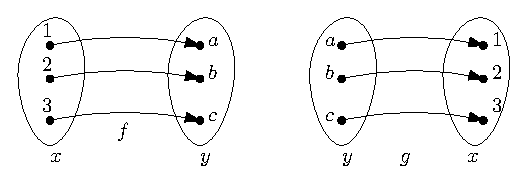
\includegraphics[width=9cm]{img/finiti/imgex4-5-1.eps}
\end{figure}

Infatti, come si vede subito, si ha
\begin{eqnarray*}
  (g\circ f)(1)=g(f(1))=g(a)=1\\
  (g\circ f)(2)=g(f(2))=g(b)=2\\ 
  (g\circ f)(3)=g(f(3))=g(c)=3
\end{eqnarray*}
Ovvero $g\circ f: \{1,2,3\}\to \{1,2,3\}$ è la funzione che manda ogni elemento dell'insieme $X=\{1,2,3\}$ in se
stesso (ovvero la funzione identica $id_x$ di $X$) e analogamente
\begin{eqnarray*}
  (f\circ g)(a)=f(g(a))=f(1)=a\\
  (f\circ g)(b)=f(g(b))=f(2)=b\\ 
  (f\circ g)(c)=f(g(c))=f(3)=c
\end{eqnarray*}
ovvero $f \circ g: \{a,b,c\}\to \{a,b,c\}$ è la funzione che manda ogni elemento dell'insieme $Y=\{a,b,c\}$ in se
stesso (cioè è la funzione identica $id_Y$).\\
Per giustificare l'affermazione che le funzioni biiettive sono le sole a essere invertibili, consideriamo ad
esempio la funzione $f$ rappresentata nel seguente disegno, che è iniettiva non suriettiva (quindi non è
biiettiva)
\begin{figure}[ht]
  \centering
  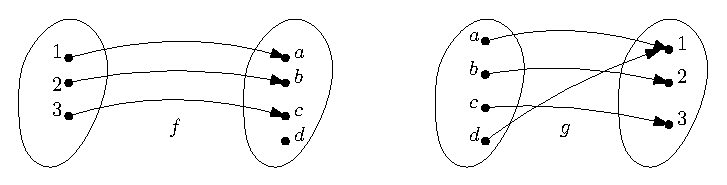
\includegraphics[width=9cm]{img/finiti/imgex4-5-2.eps}
\end{figure}

Si vede subito che $g\circ f$ è la funzione identica di $\{1,2,3\}$, ma $f\circ g$ non è la funzione identica di
$\{a,b,c,d\}$ in quanto pur essendo $f(g(a))=f(1)=a$, $f (g(b)) = f (2) = b$ e $f(g(c)) = f (3) = c$, si ha
$f(g(d))=f(1)=a$, ovvero $f\circ g$ non manda $d$ in se stesso.\\
SI osserva che non c'è alcun modo di modificare $g$ in modo che $f\circ g$ mandi ogni elemento di $\{a,b,c,d\}$
in se stesso: qualunque valore assegniato a $d$ non sarà mai $f(g(d))=d$, perché $g(d)$ dovrebbe essere un
elemento di $\{1,2,3\}$ che viene mandato da $f$ in $d$.\\
In altre parole, il motivo per cui l'ugualianza $f\circ g =id$ non può mai essere verificata è la non suriettività
è la non suriettività di $f$. Si dice che $f$ ha un'\textbf{inversa sinistra} ($g\circ f=id$ è verificato) ma non
ammette un'\textbf{inversa destra} (cioè la $f\circ g= id$ non può valere per nessuna $g$).\\
Analogamente, si prendano $f:\{1,2,3\}\to \{a,b\}$ e $g:\{a,b\}\to \{1,2,3\}$ definite come nel seguente disegno
\begin{figure}[ht]
  \centering
  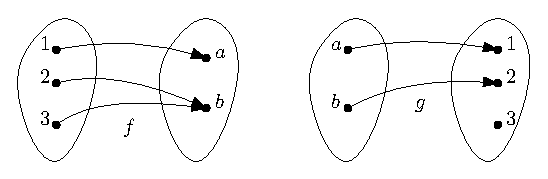
\includegraphics[width=9cm]{img/finiti/imgex4-5-3.eps}
\end{figure}

Allora, si vede subito che $f\circ g$ è la funzione identica di $\{a,b\}$, ma $g\circ f$ non è la funzione
identica di $\{1,2,3\}$ in quanto pur essendo $g(f(1))=g(a)=1$ e $g(f(2))=g(b)=2$, ovvero $g\circ f$ non manda 3
in se stesso.\\
Si osservi che anche qui non c'è alcun modo di modificare $g:$ se avessimo posto $g(b)=3$
avremmo sì ottenuto $g(f(3))=g(b)=3$ ma stavolta sarebbe stato $g(f(2))=g(b)=3$, ovvero
$g \circ f$ non avrebbe mandato 2 in se stesso: come si vede, il problema stavolta è che $f$
manda i due elementi 2 e 3 entrambi in $b$, quindi necessariamente $g(f(2))$ e $g(f(3))$ saranno
uguali e non potranno mai essere il primo 2 e il secondo 3. In altre parole, il motivo per cui
non iniettività di $f:$ la $f$ ha cioè un'inversa destra ma non un'inversa sinistra.
\begin{esempio}
  La funzione $f:\mathbb{R} \to \mathbb{R}$ data da $f(x)=x^2$, non essendo né
  iniettiva\footnote{Due numeri uno l'opposto dell'altro hanno lo stesso quadrato} né
  suriettiva\footnote{I numeri non sono quadrati di nessuno numero reale} non ha né inversa
  sinistra né inversa destra. In effetti, la condidata ad essere inversa di $f$, la radice
  quadrata $g(x)=\sqrt{x}$, da una parte non soddisfa $g(f(x))=x$ se $x$ è negativo perché in
  tal caso $g(f(x))=g(x^2)=\sqrt{x^2}=|x|$, e $|x|\neq x$ se $x$ è negativo ($|-2|=+2\neq -2$);
  dall'altra parte $f(g(y))=y$ non ha senso se $y$ è negativo in quanto in tal caso
  $g(y)=\sqrt{y}$ non è neanche un numero reale. Per eliminare i due problemi (e rendere $g$
  l'inversa di $f$) bisogna togliere i numeri negativi sia dal dominio che del codominio di $f$,
  ovvero restringerla a una funzione $f:\mathbb{R}_{\leq 0} \to \mathbb{R}_{\leq 0}$, dove
  $\mathbb{R}_{\leq 0}$ denota l'insieme dei numeri non negativi: ma così facendo in effetti
  facciamo proprio in modo che diventi una funzione biiettiva (ora non ci sono due elementi del
  dominio con lo stesso quadrato, e ogni elemento del codominio è quadrato di qualcosa).
\end{esempio}
Ora, come abbiamo detto sopra ci poniamo il problema di calcolare, se esiste, l'inversa di
un'applicazione lineare data. Prima di fare ciò, dal momento che l'inversa è definita tramite la
composizione, dobbiamo vedere cosa succede quando si compongono due applicazioni lineari.
In particolare, poiché ogni applicazione lineare può essere sempre tradotto (lavorando in
coordinate) in una funzione del tipo (4.9), vedremo cosa succede quando si compongono due
applicazioni di questo tipo.\\
Più precisamente, consideriamo $f=L_A:\mathbb{K}^n\to \mathbb{K}^m$,
\begin{eqnarray}
  \begin{matrix}
    V\to W\\
    \dim (V)=n\\
    \dim (W)=m\\
    L_A:\mathbb{K}^n\to \mathbb{K}^m
  \end{matrix} & f
                 \begin{pmatrix}
                   x_1\\
                   x_2\\
                   \vdots\\
                   x_n
                 \end{pmatrix} =
                 \begin{pmatrix}
                   a_{11}x_1+a_{12}x_2+\dots+a_{1n}x_n\\
                   a_{21}x_1+a_{22}x_2+\dots+a_{2n}x_n\\
                   \vdots\\
                   a_{m1}x_1+a_{m2}x_2+\dots+a_{mn}x_n
                 \end{pmatrix}
\end{eqnarray}
e $g=L_B:\mathbb{K}^p\to \mathbb{K}^n$
\begin{eqnarray}
  \begin{matrix}
    Z\to V\\
    \dim (Z)=p\\
    L_B:\mathbb{K}^n\to \mathbb{K}^m
  \end{matrix} & g
                 \begin{pmatrix}
                   y_1\\
                   y_2\\
                   \vdots\\
                   y_p
                 \end{pmatrix} =
                 \begin{pmatrix}
                   b_{11}y_1+b_{12}y_2+\dots+b_{1p}y_p\\
                   b_{21}y_1+b_{22}y_2+\dots+b_{2p}y_p\\
                   \vdots\\
                   b_{n1}y_1+b_{n2}y_2+\dots+b_{np}y_p
                 \end{pmatrix}
\end{eqnarray}
\begin{eqnarray*}
  \begin{matrix}
    f\circ g: & \mathbb{K}^p\stackrel{\mathrm{\color{red}g}}{\to}\mathbb{K}^n
                \stackrel{\mathrm{\color{red}f}}{\to}\mathbb{K}^m\\
    & y \mapsto g(y)\mapsto f(g(y))
  \end{matrix}
  &
    \begin{array}{cccccc}
      A & matrice & m\times m & \textit{associata ad} & f\\
      B& // & m\times p & // & g\\
      AB& // & m\times p& // &f\circ g
    \end{array}
\end{eqnarray*}
In base a quello appena visto, la composizione $f\circ g$ può essere può essere calcolata in
quento il codominio di $g$, ovvero $\mathbb{K}^n$, è anche il dominio di $f$. Si ha:
\begin{eqnarray}
  \label{eq:4.20}
  \begin{matrix}
   (f\circ g)
  \begin{pmatrix}
    y_1\\
    y_2\\
    \vdots\\
    y_p
  \end{pmatrix}=f
  \begin{pmatrix}
    g
    \begin{pmatrix}
      y_1\\
      y_2\\
      \vdots\\
      y_p
    \end{pmatrix}
  \end{pmatrix}=f
  \begin{pmatrix}
    b_{11}y_1+b_{12}y_2+\dots+b_{1p}y_p\\
    b_{21}y_1+b_{22}y_2+\dots+b_{2p}y_p\\
    \vdots\\
    b_{n1}y_1+b_{n2}y_2+\dots+b_{np}y_p
  \end{pmatrix}\\=
  \begin{pmatrix}
    a_{11}(b_{11}y_1+b_{12}y_2+\dots+b_{1p}y_p) +\dots+a_{1n}(b_{n1}y_1+b_{n2}y_2+\dots+b_{np}y_p)\\ 
    a_{21}(b_{11}y_1+b_{12}y_2+\dots+b_{1p}y_p) +\dots+a_{2n}(b_{n1}y_1+b_{n2}y_2+\dots+b_{np}y_p)\\
    \vdots\\
    a_{m1}(b_{11}y_1+b_{12}y_2+\dots+b_{1p}y_p) +\dots+a_{mn}(b_{n1}y_1+b_{n2}y_2+\dots+b_{np}y_p)
  \end{pmatrix}
  \end{matrix}
\end{eqnarray}
(raccogliendo $y_1,y_2,\dots,y_p$)
\begin{equation}
  \label{eq:4.21}
  =
  \begin{pmatrix}
    (a_{11}b_{11}+\dots+a_{1n}b_{n1})y_1+(a_{11}b_{12}+\dots+a_{1n}b_{n2})y_2+\dots+(a_{11}b_{1p}+\dots+a_{1n}b_{np})y_p\\
    (a_{21}b_{11}+\dots+a_{2n}b_{n1})y_1+(a_{21}b_{12}+\dots+a_{2n}b_{n2})y_2+\dots+(a_{21}b_{1p}+\dots+a_{2n}b_{np})y_p\\
    \vdots\\
    (a_{m1}b_{11}+\dots+a_{mn}b_{n1})y_1+(a_{m1}b_{12}+\dots+a_{mn}b_{n2})y_2+\dots+(a_{m1}b_{1p}+\dots+a_{mn}b_{np})y_p
  \end{pmatrix}
\end{equation}
Da quest'ultima espressione vediamo che la composizione $f\circ g$ è ancora una funzione del tipo
(4.9), cioè è determinata da una matrice $C$, e più precisamente
\begin{equation}
  \label{eq:4.22}
  C=
  \begin{pmatrix}
    a_{11}b_{11}+\dots+a_{1n}b_{n1}&a_{11}b_{12}+\dots+a_{1n}b_{n2}&\dots & a_{11}b_{1p}+\dots+a_{1n}b_{np}\\
    a_{21}b_{11}+\dots+a_{2n}b_{n1}&a_{21}b_{12}+\dots+a_{2n}b_{n2}&\dots & a_{21}b_{1p}+\dots+a_{2n}b_{np}\\
    &\vdots\\
    a_{m1}b_{11}+\dots+a_{mn}b_{n1}&a_{m1}b_{12}+\dots+a_{mn}b_{n2}&\dots & a_{m1}b_{1p}+\dots+a_{mn}b_{np}
  \end{pmatrix}
\end{equation}
Ora, notiamo che le entrate $c_{i1}$ di tale matrice sono tutte espressioni del tipo
\begin{equation}
  \label{eq:4.23}
  c_{ij}=a_{i1}b_{1j}+\dots+a_{in}b_{nj}
\end{equation}
in cui il primo indice dell'entrata di $A$ è fisso e sempre uguale a $i$, il secondo indice
dell'entrata di $B$ è fisso e sempre uguale a $j$ mentre gli indici ``interni''\footnote{il
  secondo dell'ntrata di $A$ e il primo dell'entrata di $B$} variano da 1 a $n$\footnote{usando
  la notazione di sommatoria, potremmo quindi scrivere $c_{ij}=\displaystyle\sum^n_{k=1}a_{ik}
  b_{kj}$}. Vedere il prodotto tra matrici (<++>).
\begin{definizione}
  La matrice $C$ le cui entrate sono date dalla (4.23) si chiama \textit{prodotto di} $A$ per
  $B$, e si scrive $C=AB$.
\end{definizione}
In pratica, abbiamo definito il prodotto di due matrici $A$ e $B$ in modo che la matriece $C=AB$
ottenuta sia la matrice che determina la composizione $L_A\circ L_B$ della funzione determinate
da $A$ e $B$.\\
Ricordando che la composizione $L_A\circ L_B$ delle due funzione $L_A$ e $L_B$ può essere fatta
solo sotto opportune condizioni\footnote{il codominio di $L_B:\mathbb{K}^p\to\mathbb{K}^n$ deve
  essere uguale al dominio di $L_A:\mathbb{K}^n\to\mathbb{K}^m$} si osserva di conseguenza che
anche il prodotto di due metrici può essere fatto solo sotto opportune condizioni: più
precisamente, del momento che la matrice di $L_A$ ha $m$ righe e $n$ colonne, mentre la matrice
$B$ di $L_B$ ha $n$ righe e $p$ colonne, vediamo che si possono moltiplicare tra loro due
matrici $A$ e $B$ (in quest'ordine) se e solo se \textit{il numero di colonne di A è uguale al
  numero di righe di B}: in tal caso, il risultato $AB$ è una matrice con $m$ righe e $n$
colonne. Se denotiamo $M_{m,n}(\mathbb{K})$ l'insieme delle matrici con $m$ righe e $n$ colonne
\footnote{Entrate appartenenti al campo $\mathbb{K}$}, possiamo allora scrivere che
\begin{equation*}
  A\in M_{m,n}(\mathbb{K}),\text{ }B\in M_{n,p}(\mathbb{K})\Rightarrow AB\in M_{m,p}(\mathbb{K})
\end{equation*}
il prodotto di matrici dato dalla Dimostrazione 4 si chiama anche \textbf{prodotto righe per
  colonna}: il motivo è che nell'espressione (4.23) della generica entrata di posto $i$ $j$
appaiono tute e sole le entrate con primo indice $i$ di $A$ e tutte e sole le entrate con
secondo indice con primo indice $i$ di $A$ e tutte e sole le entrate con secondo indice $j$ di
$B$: dal momento che il primo indice ci dice in che riga siamo, e il secondo in che colonna,
questo significa che per calcolare l'entrata di posto $i$ $j$ di $AB$ dobbiamo prendere la riga
$i$-esima di A, la $j$-esima colonna di $B$, moltiplicare tra di loro le entrate corrispondenti e
sommare il tutto
\begin{equation*}
  \begin{pmatrix}
    a_{i1} & a_{i2} &\dots & a_{in}
  \end{pmatrix}
  \begin{pmatrix}
    b_{1j}\\
    b_{2j}\\
    \dots\\
    b_{nj}
  \end{pmatrix}=
  \begin{pmatrix}
    &\dots\\
    \dots & a_{i1}b_{1j}+a_{i2}b_{2j}+\dots+a_{in}b_{nj} &\dots\\
    &\dots
  \end{pmatrix}
\end{equation*}
\begin{esempio}
  Consideriamo le due matrici
  \begin{equation*}
    A=
    \begin{pmatrix}
      1 &2\\
      4 & 5\\
      3 & 6
    \end{pmatrix} \in M_{3,2}(\mathbb{R}), \text{ } B=
    \begin{pmatrix}
      5 & 2 & 0& 1\\
      3 & 1 &-1 &2
    \end{pmatrix} M_{2,4}(\mathbb{R})
  \end{equation*}
  In base a quello che abbiamo detto, le due matrici possono essere moltiplicate e il risultato
  $AB$ sarà una matrice 3 per 4.\\
  Per trovare l'entrata di $AB$ che sta \textit{nella prima riga} e \textit{prima colonna} si
  prendono \emph{la prima riga di} $A
  \begin{pmatrix}
    1 & 2
  \end{pmatrix}
  $, \emph{la prima colonna di} $B
  \begin{pmatrix}
    5\\
    3
  \end{pmatrix}
  $, se ne moltiplicano gli elementi corrispondenti e si somma il risultato:
  $1\cdot 2 + 2\cdot 1=2+2=4$. Quindi nella prima riga, seconda colonna di $AB$ c'è
  4 -- Facendo questo calcolo su tutte le entrate, si vede che
  \begin{eqnarray*}
    AB=
    \begin{pmatrix}
      11 &4 & -2 &4\\
      35 & 13 & -5 & 14\\
      33 & 12 & -6 & 15
    \end{pmatrix}
  \end{eqnarray*}
  per maggiori chiarimento riferirsi a (<++>)
\end{esempio}
\begin{esempio}
  Come abbiamo visto nel (4.12), la matrice associata alla rotazione $f$ di angolo $\Theta$ in
   senso antiorario attorno a $O$ rispetto a una base ortogonale di $V_O^2$ è $A =
   \begin{pmatrix}
     \cos\theta & -\sin \theta\\
     \sin\theta & \cos \theta
   \end{pmatrix}
   $: la funzione $L_A:\mathbb{R}^2\to \mathbb{R}^2$ determinata da $A$, che manda $(x_1,x_2)$ in
   $(\cos \theta x_1-\sin\theta x_2,\sin\theta x_1,\cos\theta x_2)$, è la traduzione in coordinate
   di $f$. Analogamente, se $g$ denota la rotazione di angolo $\clock$, la traduzione in
   coordinate $j$ sarà data dalla funzione $L_B$ determinata dalla matrice $B=
   \begin{pmatrix}
     \cos\clock & -\sin\clock \\
     \sin \clock & \cos\clock
   \end{pmatrix}
   $. Dal momento che il prodotto di matrici ci dà la composizione della applicazioni
   corrispondenti, se moltiplichiamo $A$ e $B$ otteniamo la matrice in coordinate la
   composizione delle due rotazioni: infatti
   \begin{eqnarray*}
     AB=
     \begin{pmatrix}
       \cos\theta &-\sin\theta\\
       \sin\theta& \cos\theta
     \end{pmatrix}
     \begin{pmatrix}
       \cos\clock&-\sin\clock\\
       \sin\clock & \cos \clock
     \end{pmatrix}\\
     =
     \begin{pmatrix}
       \cos\theta\cos\clock-\sin\theta\sin\clock &-\cos\theta\sin\clock-\sin\theta\cos\clock\\
       \cos\theta \cos\clock+\cos\sin\clock & -\sin\theta\sin\clock+\cos\theta\cos\clock
     \end{pmatrix}=
   \end{eqnarray*}
   (in base alle note formule di trigonometria per il coseno e il seno della somma e della
   differenza tra due angoli)
   \begin{equation*}
     =
     \begin{pmatrix}
       \cos(\theta+\clock) &-\sin(\theta+\clock)\\
       \sin(\theta+\clock) & \cos(\theta+\clock)
     \end{pmatrix}
   \end{equation*}
   che è ancora una matrice di rotazione ma relativa all'angolo $\theta+\clock$: questo era
   prevedibile in quanto la composizione non fa altro che applicare una rotazione di angolo
   $\clock$ seguita da una rotazione di angolo $\theta$.\\
   In un capitolo successivo faremo lo stesso per calcolare la composizione di due rotazioni
   nello spazio, dove il risultato è molto meno prevedibile e intuitivo che nel caso del piano.
\end{esempio}
Vediamo ora le proprietà fondamentali del prodotto di matrici.

In primo luogo, è importatnte osservare che tale prodotto \textit{non goode della proprietà
  commutativa}, ovvero, date due matrici $A$ e $B$, e ammesso che si possano\footnote{Ad esempio,
  se $A\in M_{3,2}(\mathbb{R})$ e $B\in M_{2,4}(\mathbb{R})$, il prodotto $AB$ che $BA$ ma si
  tratta di due matrici di tipo diverso. Ad esempio, se $A\in M_{3,2}(\mathbb{R})$ e
  $B\in M_{2,3}(\mathbb{R})$ si possono eseguire entrambi i prodotti, ma $AB\in M_{3,3}
  (\mathbb{R})$ mentre $BA\in M_{2,2}(\mathbb{R})$.} eseguire entrambi i prodotti $AB$ e $BA$,
quindi non saranno in generale uquali. Ad esempio, siamo $A=
\begin{pmatrix}
  1 &2\\
  3 &4
\end{pmatrix}
$ e $B=
\begin{pmatrix}
  -1 & 0\\
  5 & 2
\end{pmatrix}
$. Allora, per definizione di prodotto righe per colonne vediamo che
\begin{eqnarray*}
  AB=
  \begin{pmatrix}
    1 &2\\
    3 &4
  \end{pmatrix}
  \begin{pmatrix}
    -1 &0\\
    5 & 2
  \end{pmatrix}=
  \begin{pmatrix}
    9& 4 \\
    17 & 8
  \end{pmatrix}\\
  BA=\begin{pmatrix}
    -1 &0\\
    5 & 2
  \end{pmatrix}
  \begin{pmatrix}
    1 &2\\
    3 &4
  \end{pmatrix}=
  \begin{pmatrix}
    -1 & -2\\
    11 & 18
  \end{pmatrix}
\end{eqnarray*}
ovvero $AB\neq BA$ --
per il prodotto tra matrici vedere (<++>).
\begin{osservazione}
  Il motivo della non commutatività in generale del prodotto di due matrici $A$ e $B$ è che,
  come sappiamo, tale prodotto rappresentala composizione delle applicazioni $L_A$ e $L_B$
  corrispondenti, e la composizione di funzioni non gode in generale della proprietà commutativa:
  ad esempio, date le due funzioni
  \begin{eqnarray*}
    f:\mathbb{R}\to \mathbb{R},\text{ } f(x)=x+1, & g:\mathbb{R}\to \mathbb{R},\text{ }g(x)=x^2
  \end{eqnarray*}
  si ha $f(g(x))=f(x^2)=x^2+1$ mentre $g(f(x))=g(x+1)=(x+1)^2$, e quindi $f\circ g\neq g\neq f$.
\end{osservazione}
Per un esempio geometrico, si considerino la funzione $f:V_O^2\to V_O^2$ che ruota ogni vettore
del piano applicato in $O$ di $90^o$ in senso antiorario, e la funzione $g:V_O^2\to V_O^2$ che
riflette ogni vettore attorno a una retta $r$ passante per $O$: allora, come si vede nel seguente
disegno, applicare prima la rotazione $f$ poi la riflessione $g$ oppure viceversa porta in
generale a risultati diversi (ovvero $f\circ g \neq g\circ f$).
\begin{figure}[ht]
  \centering
  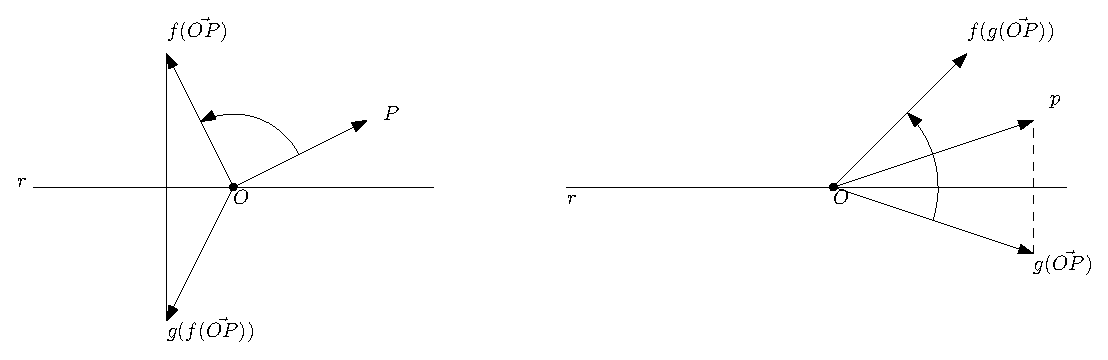
\includegraphics[width=9cm]{img/finiti/imgex4-5-4.eps}
\end{figure}

Per quello che riguarda invece la proprietà associativa, si può dimostrare che questa vale,
ovvero $(AB)C=A(BC)$. Ad esempio, siamo $A=
\begin{pmatrix}
  1 &2 \\
  3 &4
\end{pmatrix}
$,
$\begin{pmatrix}
   2 & 1\\
   -1 & 1
\end{pmatrix}$ e
$\begin{pmatrix}
   1 &5 \\
   2 &0
\end{pmatrix}$. Allora
\begin{eqnarray*}
  (AB)C=
  \begin{pmatrix}
    \begin{pmatrix}
      1 &2\\
      3 &4
    \end{pmatrix}
    \begin{pmatrix}
      2 & 1\\
      -1 & 1
    \end{pmatrix}
  \end{pmatrix}
  \begin{pmatrix}
    1 &5\\
    2 &0
  \end{pmatrix}=
  \begin{pmatrix}
    0& 3\\
    2 &7 
  \end{pmatrix}
  \begin{pmatrix}
    1 & 5\\
    2 &0
  \end{pmatrix}=
  \begin{pmatrix}
    6 &0\\
    16 & 10
  \end{pmatrix}\\
  A(BC)=
  \begin{pmatrix}
    1 &2 \\
    3 &4
  \end{pmatrix}
  \begin{pmatrix}
     \begin{pmatrix}
      2 & 1\\
      -1 & 1
    \end{pmatrix}
    \begin{pmatrix}
      1 &5\\
      2 &0
    \end{pmatrix}  
  \end{pmatrix}=
  \begin{pmatrix}
    1 &2 \\
    3 &4
  \end{pmatrix}
  \begin{pmatrix}
    4 &10\\
    1 & -5
  \end{pmatrix}=
  \begin{pmatrix}
    6 &0\\
    16 & 10
  \end{pmatrix}
\end{eqnarray*}
\begin{osservazione}
  l’associatività del prodotto di matrici si spiega facilmente ricordando che tale
  prodotto rappresenta la composizione delle funzioni corrispondenti, ovvero $(AB)C$ rappresenta
  $(L_A\circ L_B)\circ L_C$ mentre $A(BC)$ rappresenta $L_A\circ (L_B\circ L_C)$. Ma è facile
  vedere che la composizione di funzioni gode della propriet`a associativa: infatti, applicando
  $(f\circ g)\circ h$ a $x$ otteniamo $(f\circ g)(h(x))=f(g(h(x)))$, e analogamente applicando
  $f\circ(g\circ h)$ a $x$ otteniamo sempre $f((g\circ h)(x))=f(g(h(x)))$, ovvero $(f\circ g)
  \circ h= f\circ (g\circ h)$.
\end{osservazione}
Ci chiediamo ora se il porodotto di matrice ammetta un elemento neutro che svolga lo stesso
ruolo che svolge il numero 1 per il prodotto tra numeri, per cui si ha $a \cdot 1 =1 \cdot a=a$
per ogni numero $a$. La risposta è affermativa: più precisamente, per ogni $n$ consideriamo la
matrice con $n$ righe e $n$ colonne seguente
\begin{equation}
  \begin{pmatrix}
    1 & 0 &\dots &0\\
    0 &1 &\dots& 0\\
      && \vdots\\
    0& 0&\dots&1
  \end{pmatrix}
\end{equation}
ovvero la matrice che ha 1 nelle entrate con stesso indice di riga e di colonna $(a_{11},a_{22},etc.)$ e 0 in tutte le altre entrate. Tale matrice si chiama \emph{matrice identica di ordine n e
  e si denota $I_n$.} Ad esempio,
\begin{equation*}
  I_2=
  \begin{pmatrix}
    1 &0\\
    0 &1
  \end{pmatrix}, \text{ }
  I_3=
  \begin{pmatrix}
    1 &0&0\\
    0&1&0\\
    0&0&1
  \end{pmatrix}
\end{equation*}
\begin{osservazione}
  In generale, data una matrice quadrata di ordine $n$, le entrate $a_{11}, a_{22}, a_{nn}$ che
  hanno lo stesso indice di riga e di colonna formano la cosiddetta \textit{diagonale della
    matrice}. la matrice identica $I_n$ può essere quindi descritta come la matrice che ha 1
  sulla diagonale e 0 nelle altre entrate. Le entrate di $I_n$ si denotano solitamente con il
  simbolo $\delta_{ij}$, detto \textit{delta di Kroneeker}\footnote{Il delta di Kronecker è una
    funzione di due variabili, di solito solo numeri interi non negativi. La funzione è 1 se le
    variabili sono uguali e 0 atrimenti: $\delta_{ij}=
    \begin{cases}
      0 & \text{se } i\neq j,\\
      1 & \text{se } i = j.
    \end{cases}$ o con l'uso di staffe Iverson: $\delta_{ij}=[i=j]$ dove il delta di Kronecker
    $\delta_{ij}$ è una funzione a tratti delle variabili $i$ e $j$.}.
  Ora, si puà verificare che, per ogni $A\in M_{m,n}(\mathbb{K})$ si ha
  \begin{equation*}
    AI_n=A, \text{ } I_mA=A.
  \end{equation*}
  e quindi la matrice identica svolge esattametne il ruolo di elemento neutro per il prodotto
  righe per colonne. Ad esempio,
  \begin{eqnarray*}
    \begin{pmatrix}
      1 &2&3\\
      4 &5 & 6
    \end{pmatrix}  \begin{pmatrix}
      1 &0&0\\
      0&1&0\\
      0&0&1
                   \end{pmatrix}
    =
    \begin{pmatrix}
      1 & 2& 3\\
      4 & 5 & 6
    \end{pmatrix}\\
    \begin{pmatrix}
      1 &0\\
      0 &1
    \end{pmatrix} 
    \begin{pmatrix}
      1 & 2& 3\\
      4 & 5 & 6
    \end{pmatrix}=
    \begin{pmatrix}
      1 & 2& 3\\
      4 & 5 & 6
    \end{pmatrix}
  \end{eqnarray*}
\end{osservazione}
\begin{osservazione}
  Si noti che la matrice indetica $I_n$ non è nient'altro che la matrice che determina la
  funzione identica $id_{\mathbb{K}^n}:\mathbb{K}^n\to \mathbb{K}?n$ che manda ongi elemento in se
  stesso: infatti,
  \begin{equation}
    id_{\mathbb{K}^n}
    \begin{pmatrix}
      x_1\\
      x_2\\
      \vdots\\
      x_n
    \end{pmatrix}=
    \begin{pmatrix}
      x_1\\
      x_2\\
      \vdots\\
      x_n
    \end{pmatrix}=
    \begin{pmatrix}
      1x_1+0x_2+\dots+0x_n\\
      0x_1+1x_2+\dots+0x_n\\
      \vdots\\
      0x_1+0x_2+\dots+1x_n
    \end{pmatrix}
  \end{equation}
  Questo spiega perché tale matrice sia l'elemento neutro per il prodotto, in quanto il
  prodotto tra matrici rappresenta la composizione delle applicazioni corrispondenti e la funzione identica è
  esattamente l'elemento neutro per la composizione.
\end{osservazione}
Continuando con l'analogo con il prodoto tra numeri, vogliamo ora esaminare la questione
dell'esistenza la questione \textit{dell'esistenza dell'inverso}: come sappiamo, nell'insieme dei numeri reali
$\mathbb{R}$ per pgni numero $a$ diverso da zero esiste un numero $b$ tale che $ab-ba=1$, detto appunto inverso
di $a$ (e denotato $a^{-1}$).\\
Nel caso delle matrici, verremmo quindi capire se data una matrice $A\in M_{m,n} (\mathbb{K})$ esiste una
matrice\footnote{la scelta del numero di righe e di colonne di $B$ è obbligata se vogliamo poter eseguire sia il
prodotto $AB$ che quello $BA$} $B\in M_{n,m}(\mathbb{K})$ tale che
$AB=I_m$ e $BA=I_n$. Tuttavia, se una tale $B$ esiste, dal momento che il prodotto di $A$
e $B$ corrisponde alla composizione della applicazione lineare $L_A:\mathbb{K}^n\to \mathbb{K}$ e si ha
$L_A\circ L_B=id$ e $L_B\circ L_A=id$, ovvero la funzione $L_A$ deve essere invertibile. Ma allora, come abbiamo
visto in \ref{Composizione di applicazioni, inversa e prodotto di matrici}, $L_A:\mathbb{K}^n\to \mathbb{K}^m$
deve essere biiettiva, il che in base al Corollario <++> è possibile solo se il dominio e il codominio hanno
la stessa dimensione, ovvero solo se $m=n$.\\
Riassumendo, abbiamo mostrato che il problema dell'inverso si pone solo per matrici che hanno stesso numero di
righe e di colonne, ovvero solo se $A\in M_{n,n}(\mathbb{K})$. Tali matrici si dicono \emph{quadrate} e il
numero $n$ comune di righe e colonne si dice \emph{ordine della matrice}. Per semplicità, l'insieme $M_{n,n}
(\mathbb{K})$ si denota $M_n(\mathbb{K})$. Diamo allora la seguente
\begin{definizione}
  Una matrice $A\in M_n(\mathbb{R})$ quadrata di ordine $n$ si dice \textit{invertibile} se matrice $B\in M_n
  (\mathbb{K})$ tale che
  \begin{eqnarray}
    AB=I_n, & BA=I_n
  \end{eqnarray}
  In tal caso, $B$ si chiama \textit{matrice inversa di} $A$ e si denota $A^{-1}$.
\end{definizione}
\begin{itemize}
\item Una matrice invertibile si può anche chiamare \texttt{NON SINGOLARE}
\item Una matrice non invertibile si può anche chiamare \texttt{SINGOLARE}
\end{itemize}
\clearpage
Dimostriamo ora il seguente risultato, che ci dice che, contrariamente a quello che accade nel campo dei numeri
reali dove l'unità numero non invertibile è lo zero, nell'insieme delle matrici, anche limitandosi alle sole
matrici quadrate, ci sono molte matrici non invertibili:
\begin{teorema}
  Una matrice $A\in M_n(\mathbb{K})$ è invertibile se e solo se il rango di $A$ è uguale a $n$.
\end{teorema}
\begin{proof}
  Come abbiamo ricordato poco prima della Definizione <++>, l'invertibilità di $A$, ovvero l'esistenza di una
  matrice $B$ tale che $AB=BA=I_n$, equivale a dire $L_A\circ L_B=L_B\circ L_A=id$, ovvero che $L_A$ è
  invertibile\footnote{Volendo essere rigorosi, essere rigorosi, $L_A\circ L_B=L_B\circ L_A=id$ implica
    chiaramente che $L_A$ sua invertibile, ma vicersa il fatto che $L_A$ sia invertibile implica solo che esista
    una funzione $g$ tale che $g\circ L_A=L_A\circ g =id$, che a priori non sappiamo se è della forma $g=L_B$ per
    qualche matrice $B$. In realtà, si può dimostrare che $g$ deve necessariamente essere di quella forma, e
    quindi otteniamo anche l'implicazione opposta per cui $L_A$ invertibile implica che esiste una matrice $B$
    per cui $g\circ L_A\circ L_B=L_B\circ L_A =id$ (e quindi $AB=BA=I_n$).} e quindi biiettiva. Quindi ci basta
  dimostrare $L_A$ sia biiettivo se e solo se il rango di $A$ è $n$. Ora, come abbiamo visto nel Corollario <++>,
  una funzione lineare in cui dominio e codominio abbiano la stessa dimensione\footnote{e $L_A: \mathbb{K}^n\in
    \mathbb{K}^n$ verifica questa condizione} iniettiva se e solo se è suriettiva, ovvero basta una delle due
  proprietà per avere anche l'altra entrambe le proprietà (e quindi la biiettività) è necessaria e sufficiente
  che una delle due venga soddisfatta. Quindi, possiamo dire che $L_A$ è biiettiva solo se è suriettiva.
  Ma come abbiamo visto in \ref{sec:inie_surie_app_lin_ric_gen}, $L_A$ è suriettiva se e solo se il rango
  di $A$ è $n$. 
\end{proof}
Vediamo ora come si calcola l'inversione di una matrice $A$, suponendo che questa esita (cioè che $A$ sia
invertibile).\\
Quindi siamo pronti a trattare il primo metodo d'inversione di una matrice: sappiamo che trovare l'inversa
di $A$ equivale a trovare una matrice $B$ tale che $AB=I_n$ (senza dever verificare anche $BA=I_n$), ovvero
\begin{equation*}
  \begin{pmatrix}
    a_{11} &a_{12} &\dots & a_{1n}\\
    a_{21} & a_{22} & \dots & a_{2n} \\
           && \dots\\
    a_{n1} & a_{n2} & \dots&a_{nn}
  \end{pmatrix}
  \begin{pmatrix}
    b_{11} &b_{12} &\dots & b_{1n}\\
    b_{21} & b_{22} & \dots & b_{2n} \\
           && \dots\\
    b_{n1} & b_{n2} & \dots&b_{nn}
  \end{pmatrix}=
  \begin{pmatrix}
    1 &0 &\dots&0\\
    0 & 1 &\dots & 0\\
      &&\dots\\
    0 & 0&\dots & 1
  \end{pmatrix}
\end{equation*}
Tenuto conto della dimostrazione di prodotto righe per colonne, vediamo che moltplicando le riche di $A$ per la
prima colonna di $B$ deve essere
\begin{equation*}
  \begin{cases}
    a_{11}b_{11} + a_{12}b_{21}+\dots +a_{1n}b_{n1} =1\\
    a_{21}b_{11} + a_{22}b_{21}+\dots +a_{2n}b_{n1} =0\\
    \dots\\
    a_{n1}b_{11} + a_{n2}b_{21}+\dots +a_{nn}b_{n1} =0
  \end{cases}
\end{equation*}
ovvero la prima colonna di $B$ soddisfa il sistema
\begin{equation}
   \begin{cases}
    a_{11}x_1 + a_{12}x_2+\dots +a_{1n}x_n =1\\
    a_{21}x_1 + a_{22}x_2+\dots +a_{2n}x_n =0\\
    \dots\\
    a_{n1}x_1 + a_{n2}x_2+\dots +a_{nn}x_n =0
  \end{cases}
\end{equation}
con matrice dei coefficienti uguale a $A$ e termini noti uguali alla prima colonna della matrice identica.\\
Analogamente, moltiplicando le righe di $A$ per la seconda colonna di $B$ si vede che devono essere soddisfatte
le sequenti
\begin{equation*}
  \begin{cases}
    a_{11}b_{12} + a_{12}b_{22}+\dots +a_{1n}b_{n2} =0\\
    a_{21}b_{12} + a_{22}b_{22}+\dots +a_{2n}b_{n2} =1\\
    \dots\\
    a_{n1}b_{12} + a_{n2}b_{22}+\dots +a_{nn}b_{n2} =0
  \end{cases}
\end{equation*}
ovvero la seconda colonna di $B$ deve soddisfare il sistema
\begin{equation}
   \begin{cases}
    a_{11}x_1 + a_{12}x_2+\dots +a_{1n}x_n =0\\
    a_{21}x_1 + a_{22}x_2+\dots +a_{2n}x_n =1\\
    \dots\\
    a_{n1}x_1 + a_{n2}x_2+\dots +a_{nn}x_n =0
  \end{cases}
\end{equation}
sempre con matrice dei coefficienti uguale a $A$ ma stavolta con temini noti uguali alla matrice identica, e
così via possiamo ragionare allo stasso fino all'ultima colonna di $B$ che dovrà soddisfare
\begin{equation*}
  \begin{cases}
    a_{11}b_{1n} + a_{12}b_{2n}+\dots +a_{1n}b_{nn} =0\\
    a_{21}b_{1n} + a_{22}b_{2n}+\dots +a_{2n}b_{nn} =1\\
    \dots\\
    a_{n1}b_{1n} + a_{n2}b_{2n}+\dots +a_{nn}b_{nn} =0
  \end{cases}
\end{equation*}
ovvero il sistema
\begin{equation}
   \begin{cases}
    a_{11}x_1 + a_{12}x_2+\dots +a_{1n}x_n =0\\
    a_{21}x_1 + a_{22}x_2+\dots +a_{2n}x_n =0\\
    \dots\\
    a_{n1}x_1 + a_{n2}x_2+\dots +a_{nn}x_n =1
  \end{cases}
\end{equation}
Riassumendo, si ha $AB=I_n$ se e solo se le colonne $
\begin{pmatrix}
  b_{11}\\
  b_{21}\\
  \dots\\
  b_{n1}
\end{pmatrix},
\begin{pmatrix}
  b_{12}\\
  b_{22}\\
  \dots\\
  b_{n2}
\end{pmatrix},
\begin{pmatrix}
  b_{1n}\\
  b_{2n}\\
  \dots\\
  b_{nn}
\end{pmatrix}
$ sono soluzione rispettivamente degli $n$ sistemi (4.27), (4.28), \dots, (4.29).\\
Come sappiamo, per risolvere un sistema basta scriverne la matrice completa, composta da matrice dei
coefficienti delle incognite e colonne dei termini noti, e ridurla a gradini mediamente operazioni elementari
sulle righe. Poiché i sistemi (4.27), (4.28), \dots, (4.29) hanno tutti la stessa matrice dei coefficienti, cioè
$A$, e differiscono solo per i termini noti, possiamo risolverli tutti contemporaneamente eseguendo le stesse
operazioni elementari: a questo scopo, basta scriver la matrice
\begin{equation}
  \label{eq:4.30}
  (A|I_n)=\left(
    \begin{array}[center]{cccc|cccc}
      a_{11} & a_{12} & \dots & a_{1n} & 1 & 0 & \dots &0\\
      a_{21} & a_{22} & \dots & a_{2n} & 0 & 1 & \dots &0\\
      a_{n1} & a_{n2} & \dots & a_{nn} & 0 & 0 & \dots &1 
    \end{array}
    \right)
\end{equation}
ottenuta affiacando tutti i termini noti dei sistemi (4.27), (4.28), \dots, (4.29) e risolverli
contemporaneamente con una sola riduzione\footnote{chiaramente, in base al Teorema <++> la matrice A è
  invertibile se e solo se in seguito a tale riduzione non si annullarà nessuna delle sue righe}.\\
Vediamo subito un esempio: dato la matrice $A=
\begin{pmatrix}
  1 & -1\\
  1 & 2
\end{pmatrix}
$, verifichiamo se essa è invertibile e, in caso affermativo, calcoliamo l'inversa. Come detto sopra,
affianchiamo a tale matrice la matrice identica dello stesso ordine
\begin{equation*}
  (A|I_n)=\left(
  \begin{array}{cc|cc}
    1&-1&1&0\\
    1&2&0&1
  \end{array}\right)
\end{equation*}
che rappresenta i due sistemi le cui soluzioni sono le colonne della matrice inversa, e iniziamo con
l'applicare il procedimeto di riduzione a gradini: a questo scopo basta il singolo passaggio
\begin{equation}
  \label{eq:4.31}
  (A|I_n)=\left(
  \begin{array}{cc|cc}
    1&-1&1&0\\
    1&2&0&1
  \end{array}\right) \underset{R_2\to R_2-R_1}{\to} \left(
  \begin{array}[center]{cc|cc}
    1 &-1 & 1 &0\\
    0 & 3 & -1 &1
  \end{array}\right)
\end{equation}
da cui vediamo che, dopo la riduzione a gradini, ad $A$ non si annulla nessuna riga e quindi, come abbiamo detto
sopra, $A$ è invertibile.\\
La prima colonna dell'inversa $B$ di $A$ è data dalla soluzione del sistema ridotto
\begin{equation}
  \label{eq:4.32}
  \begin{cases}
    x_1-x_2=1\\
    3x_2=1
  \end{cases}
\end{equation}
ovvero, come si vede risolvendo dal basso, la coppia $\left(\frac{2}{3},\frac{1}{3}\right)$, che è quindi
la prima colonna della matrice inversa. Analogamente, la seconda colonna dell'inversa $B$ di $A$ è data della
soluzione del sistema ridotto
\begin{equation}
  \label{eq:4.33}
  \begin{cases}
    x_1-x_2=0\\
    3x_2=1
  \end{cases}
\end{equation}
ovvero, come si vede risolvendo dal basso, la coppia $\left(\frac{1}{3},\frac{1}{3}\right)$, che è quindi la
seconda colonna della matrice inversa. In conclusione, l'inversa dell matrice $A$ è
\begin{equation*}
  A^{-1}=
  \begin{pmatrix}
    \frac{2}{3} &\frac{1}{3}\\
    -\frac{1}{3} & \frac{1}{3}
  \end{pmatrix}
\end{equation*}
Infatti, si verifica subito con un calcolo che 
\begin{equation*}
  \begin{pmatrix}
    1 & -1\\
    1 & 2
  \end{pmatrix}
  \begin{pmatrix}
     \frac{2}{3} &\frac{1}{3}\\
    -\frac{1}{3} & \frac{1}{3}
  \end{pmatrix}=
   \begin{pmatrix}
     \frac{2}{3} &\frac{1}{3}\\
    -\frac{1}{3} & \frac{1}{3}
   \end{pmatrix}
   \begin{pmatrix}
    1 & -1\\
    1 & 2
   \end{pmatrix}=
   \begin{pmatrix}
     1 &0\\
     0 &1
   \end{pmatrix} 
\end{equation*}
concordemente con la definizione di inversa.\\
Per evitare di scrivere e risolvere separatamente i sistemi (\ref{eq:4.32}) e (\ref{eq:4.33}), e trovare invece in
modo più diretto la matrice inversa, si può procedere come segue. Dopo per effettuato la riduzione a gradini in
(\ref{eq:4.31}), si applicano ulteriori operazioni elementari fino a trasformare la matrice $A$ del blocco di
sinistra nella matrice identica: a questo punto nel blocco di destra si legge direttamente l'inversa. Per vederlo,
riprendiamo da (\ref{eq:4.31}) e facciamo comparire prima uno zero in posizione 1 2 eseguendo
\begin{equation*}
  \left(
  \begin{array}{cc|cc}
    1&-1&1&0\\
    0&3&-1&1
  \end{array}\right) \underset{R_2\to R_2-R_1}{\to} \left(
  \begin{array}[center]{cc|cc}
    3 & 0 & 2 &1\\
    0 & 3 & -1 &1
  \end{array}\right)
\end{equation*}
e applichiamo poi a ogni riga l'operazione elementare del secondo tipo che consiste nel dividerla per l'elemento
che si trova sulla diagonale:
\begin{equation}
  \label{eq:4.34}
  \left(
  \begin{array}[center]{cc|cc}
    3 & 0 & 2 &1\\
    0 & 3 & -1 &1
  \end{array}\right)
\underset{
  \begin{matrix}
    R_1\to (1/3) R_1\\ R_2\to(1/3) R_2
  \end{matrix}}{\to}
  \left(
  \begin{array}[center]{cc|cc}
    1 & 0 & 2/3 &1/3\\
    0 & 1 & -1/3 &1/3
  \end{array}\right) 
\end{equation}
Come si vede la matrice identica che avevamo affiancato ad $A$ si è trasformata nella matrice inversa di
$A$ già trovata sopra.\\
Per capire perché, ricordiamo che le operazioni elementari che stiamo eseguendo servono a risolvere
contemporaneamente  poi ci danno come soluzione le colonne della matrice inversa: ma allora, riducendo la matrice
$A$\footnote{cioè la matrice dei coefficienti di tali sistemi} alla matrice identica come in (\ref{eq:4.34}) non
non stiamo facendo altro che ridurre i due sistemi alla forma
\begin{eqnarray*}
  \begin{cases}
    x_1=\frac{2}{3}\\
    x_2=-\frac{1}{3}
  \end{cases}
  &,&
      \begin{cases}
        x_1=\frac{1}{3}\\
        x_2=\frac{1}{3}
      \end{cases}
\end{eqnarray*}
e cioè far comparire direttamente le soluzioni cercate (che sono proprio le colonne della matrice inversa).\\
Vediamo un altro esempio:
\begin{eqnarray*}
  A=\begin{pmatrix}
      1 &1 &2\\
      -1 & 1 &0\\
      2 & 1 &1
  \end{pmatrix}.
\end{eqnarray*}
Iniziamo con il trasformare la matrice $(A|I_n)$ in una matrice a gradini
\begin{equation*}
  (A|I_n)=
  \left(
  \begin{array}[center]{ccc|ccc}
    1 & 1 & 2 &1 &0&0\\
    -1 & 1 &0 & 0&1&0\\
    2 &1 &1&0&0&1
  \end{array}\right)
  \underset{
  \begin{matrix}
    R_1\to R_2+R_1\\ R_3\to  R_3-2R_1
  \end{matrix}}{\to}
  \left(
  \begin{array}{ccc|ccc}
     1 & 1 & 2 &1 &0&0\\
    0 & 2 &2 & 1&1&0\\
     0 & -1 &-3&-2&0&1
  \end{array}\right)
\end{equation*}
\begin{equation*}
  \left(
  \begin{array}{ccc|ccc}
     1 & 1 & 2 &1 &0&0\\
    0 & 2 &2 & 1&1&0\\
     0 & -1 &-3&-2&0&1
  \end{array}\right)
  \underset{
  \begin{matrix}
    R_3\to 2R_3+R_2
  \end{matrix}}{\rightarrow} 
  \left(
  \begin{array}{ccc|ccc}
     1 & 1 & 2 &1 &0&0\\
    0 & 2 &2 & 1&1&0\\
     0 & 0 &-4&-3&1&2
  \end{array}\right)
\end{equation*}
Il fatto che non si sia annullata nessuna riga nel blocco di sinistra ci dice che la matrice $A$ è invertibile.\\
Ora, come spiegato sopra, faciamo comparire zeri sopra la diagonale, effettuando una sorta di riduzione a gradini
``all'incontrario'', dal basso verso l'altro e da destra verso sinistra\footnote{in ogni passaggio, mettiamo in
  evidenza in grasseto i nuivi zeri che facciamo comparire}
\begin{equation*}
   \left(
  \begin{array}{ccc|ccc}
     1 & 1 & 2 &1 &0&0\\
     0 & 2 &2 & 1&1&0\\
     0 & 0 &-4&-3&1&2
  \end{array}\right)
   \underset{
  \begin{matrix}
    R_2\to 2R_2+R_3\\ R_1\to  2R_1-R_3
  \end{matrix}}{\to}
   \left(
  \begin{array}{ccc|ccc}
     2 & 2 & \mathbf{0} &-1 &1&2\\
     0 & 4 &\mathbf{0} & 1&3&2\\
     0 & 0 &-4&-3&1&2
  \end{array}\right)
\end{equation*}
\begin{equation*}
    \left(
  \begin{array}{ccc|ccc}
     2 & 2 & \mathbf{0} &-1 &1&2\\
     0 & 4 &\mathbf{0} & 1&3&2\\
     0 & 0 &-4&-3&1&2
  \end{array}\right)
   \underset{
  \begin{matrix}
    R_1\to  2R_1-R_3
  \end{matrix}}{\to}
    \left(
  \begin{array}{ccc|ccc}
     4 & \mathbf{0} & 0 &-1 &-1&2\\
     0 & 4 &0 & -1&3&2\\
     0 & 0 &-4&-3&1&2
  \end{array}\right)
\end{equation*}
Infatti, dividiamo ogni riga per l'elemento sulla diagonale applicando operazioni elementari del secondo tipo
\begin{equation*}
     \left(
  \begin{array}{ccc|ccc}
     4 & 0 & 0 &-1 &-1&2\\
     0 & 4 &0 & -1&3&2\\
     0 & 0 &-4&-3&1&2
  \end{array}\right)
   \underset{
  \begin{matrix}
    R_1\to (1/4)R_1\\
    R_1\to (1/4)R_2\\
    R_3\to (1/4)R_3
  \end{matrix}}{\to}
\left(
  \begin{array}{ccc|ccc}
    1&0&0&-\frac{1}{4}&-\frac{1}{4}&\frac{1}{2}\\
    0&1&0&-\frac{1}{4}&-\frac{3}{4}&\frac{1}{2}\\
    0 & 0 &1 &\frac{3}{4}&-\frac{1}{4}&-\frac{1}{2}
  \end{array}\right)
\end{equation*}
Quindi
\begin{equation*}
  A^{-1}=
  \begin{pmatrix}
    -\frac{1}{4}&-\frac{1}{4}&\frac{1}{2}\\
    -\frac{1}{4}&-\frac{3}{4}&\frac{1}{2}\\
    \frac{3}{4}&-\frac{1}{4}&-\frac{1}{2}
  \end{pmatrix}
\end{equation*}
Vediamo ora un modo alternativo per calcolare l'inversa di una matrice invertibile, basato sul determinante e
sulla nozione di cofattore, vista nel precedente capitolo.\\
Abbiamo visto nel Teorema <++> che una matrice $A$ di ordine $n$ è invertibile se e solo se il suo rango è $n$.
Ma come sappiamo dal Teorema <++>, questo equivale ad avere $\det(A)\neq 0$. Dimostriamo ora la seguente
\begin{proposizione}
  Sia $A\in M_n(\mathds{K})$ una matrice invertibile\footnote{ovvero con $\det(A)\neq 0$}. Allora la sua inversa
  $A^{-1}$ è data da
  \begin{equation}
    \label{eq:4.35}
    A^{-1}=\frac{1}{\det (A)}
    \begin{pmatrix}
      C_{11} &C_{21}&\dots & C_{n1}\\
      C_{12} &C_{22}&\dots & C_{n2}\\
      & \dots\\
      C_{1n} & C_{2n} &\dots & C_{nn}
    \end{pmatrix}
  \end{equation}
  dove $C_{ij}$ indica il cofattore di $a_{ij}$, e $\frac{1}{\det(A)}$ davanti alla matrice dei cofattori
  significa che ogni entrata di tale matrice deve essere moltiplicato per $\frac{1}{\det (A)}$.
\end{proposizione}
\begin{osservazione}
  \label{oss:10}
  A proposito della disposizione dei cofattori nella (\ref{eq:4.35}), si noti che i cofattori delle entrate della
  prima \textit{riga} di $A$ sono nella prima \textit{colonna} della (\ref{eq:4.35}), i cofattori delle entrate
  della della seconda $riga$ di $A$ sono nella seconda \textit{colonna} della (\ref{eq:4.35}), e così via.
\end{osservazione}
\begin{esempio}
  Calcoliamo l'inversa della matrice $A=
  \begin{pmatrix}
    1 & 2 &1\\
    1 & -1 & 1\\
    1 & 0 &2
  \end{pmatrix}
  $.\\
  I cofattori sono
  \begin{eqnarray*}
    C_{11}=(-1)^{1+1}\det
    \begin{pmatrix}
      -1 & 1 \\
      1 & 0
    \end{pmatrix}
    =-2, & C_{12}=(-1)^{1+2}\det
                            \begin{pmatrix}
                              1 & 1 \\
                              1 &2
                            \end{pmatrix}=-1\\
     C_{13}=(-1)^{1+3}\det
    \begin{pmatrix}
      1 & -1 \\
      1 & 0
    \end{pmatrix}
    =1, & C_{21}=(-1)^{2+1}\det
                            \begin{pmatrix}
                              1 & 2 \\
                              1 &0
                            \end{pmatrix}=-4\\
    C_{22}=(-1)^{2+2}\det
    \begin{pmatrix}
      1 & 1 \\
      1 & 2
    \end{pmatrix}
    =1, & C_{23}=(-1)^{3+2}\det
                            \begin{pmatrix}
                              1 & 1 \\
                              1 &1
                            \end{pmatrix}=0\\
    C_{31}=(-1)^{3+1}\det
    \begin{pmatrix}
      2 & 1 \\
      -1 & 1
    \end{pmatrix}
    =3, & C_{32}=(-1)^{3+2}\det
                            \begin{pmatrix}
                              1 & 1 \\
                              1 &1
                            \end{pmatrix}=0
  \end{eqnarray*}
  \begin{equation*}
    C_{11}=(-1)^{3+3}\det
    \begin{pmatrix}
      1 & 2 \\
      1 & -1
    \end{pmatrix}
    =-3.
  \end{equation*}
  Quindi
  \begin{equation*}
    A^{-1}=\frac{1}{\det(A)}
    \begin{pmatrix}
      C_{11} & C_{21} & C_{31}\\
      C_{12} & C_{22} & C_{32}\\
      C_{13} & C_{2n} & C_{33}
    \end{pmatrix}=-\frac{1}{3}
    \begin{pmatrix}
      -2 & -4 & 3\\
      -1 & 1 &0\\
      1 & 2 & -3 
    \end{pmatrix} =
    \begin{pmatrix}
      \frac{2}{3} & \frac{4}{3} & -1\\
      \frac{1}{3} & -\frac{1}{3} & 0\\
      -\frac{1}{3} & -\frac{2}{3} & 1
    \end{pmatrix}.
  \end{equation*}
  dove il determinante di $A$ è stato calcolato sviluppandolo secondo Laplace rispetto alla tesza riga, usando i
  cofattori già calcolati:
  \begin{equation*}
    \det (A)=a_{31}C_{31}+a_{32}C_{32} +a_{33}C_{33} = 1\cdot 3 + 0\cdot 0 + 2\cdot (-3)=-3
  \end{equation*}
\end{esempio}
\begin{osservazione}
  Osservando che la \ref{eq:4.35}, nel caso $n=2$, diventa la semplice formula
  \begin{equation}
    \label{eq:4.40}
    \begin{pmatrix}
      a_{11} & a_{12}\\
      a_{21} & a_{22}
    \end{pmatrix}^{-1}=\frac{1}{a_{11}a_{22}-a_{12}a_{21}}
    \begin{pmatrix}
      a_{22} & -a_{12}\\
      -a_{21} & a_{11}
    \end{pmatrix}.
  \end{equation}
  in quanto i cofattori sono semplicemente $C_{11}=(-1)^{1+1}a_{22},\text{ } C_{12}=(-1)^{1+2}a_{21},
  C_{21}=(-1)^{2+1}a_{12},$\\ $\text{ } C_{22}=(-1)^{2+2}a_{11}$ (ricordiamo che il determinante di una matrice di
  ordine 1 si definisce come il valore della sua unica entrata). In pratica, a parte dividere per il
  determinante, la matrice inversa si ottiene scambiando tra loro i due elementi sulla diagonale e cambiando di
  segno le restanti entrate.
\end{osservazione}
\begin{esempio}
  Applichiamo la (\ref{eq:4.40}) al caso della matrice che rappresenta una rotazone di angolo $\theta$ nel piano,
  ovvero $A=
  \begin{pmatrix}
    \cos\theta&-\sin \theta\\
    \sin\theta&\cos \theta
  \end{pmatrix}
  $: si ha
  \begin{equation*}
    A^{-1}=\frac{1}{\cos^2\theta+\sin^2\theta}
  \begin{pmatrix}
    \cos\theta&\sin \theta\\
    -\sin\theta&\cos \theta
  \end{pmatrix}
\end{equation*}
(per l'identità $\cos^2\theta+\sin^2\theta=1$ e le formule trigonometriche per il seno e il coseno dell'opposto
di un angolo)
\begin{equation*}
  =
  \begin{pmatrix}
    \cos(-\theta) & -\sin(-\theta)\\
    \sin(-\theta) & \cos(-\theta)
  \end{pmatrix}
\end{equation*}
che è ancora una matrice di rotazione, quella associata alla rotazione di angolo $-\theta$, che è l'inversa della
rotazione di angolo $\theta$\footnote{se applichiamo prima una e poi l'altra il vettore torna alla posizione
  iniziale}.\\
In effetti, in generale, la matrice $A^{-1}$ inversa di una matrice $A$ data rappresenta la funzione della
funziona inversa della funzione $L_A:\mathds{K}^n\to\mathds{K}^n$ determinante da $A$: infatti, come sappiamo la
composizione $L_A\circ L_{A^{-1}}=id$ (e analogamente $L_{A^{-1}} \circ L_A=id$).
\end{esempio}
Vediamo ora che la formula (\ref{eq:4.35}) per il calcolo dell'inversa può essere utilizzata per ricavare un modo
alternativo alla riduzione a gradini per risolvere certi sistemi di equazioni lineari.\\
A tale scopo, osserviamo prima che un generico sistema lineare di $m$ equazioni in $n$ incognite.
\begin{equation}
  \label{eq:3.37}
  \begin{cases}
    a_{11}x_1+a_{12}x_2+\dots+a_{1n}x_n=b_1\\ 
    a_{21}x_1+a_{22}x_2+\dots+a_{2n}x_n=b_2\\
    \vdots\\
    a_{m1}x_1+a_{m2}x_2+\dots+a_{mn}x_n=b_m
  \end{cases}
\end{equation}
può essere riscitto in forma molto più concisa grazie al prodotto di matrici. Più precisamente, se denotiamo con
$A=
\begin{pmatrix}
  a_{11} & a_{12} & \dots & a_{1n}\\
  a_{21} & a_{22} & \dots & a_{2n}\\
         &\vdots\\
  a_{m1} & a_{m2} & \dots & a_{mn}
\end{pmatrix}
$ la matrice dei coefficiati del sistema, con $x=
\begin{pmatrix}
  x_1\\
  x_2\\
  \vdots\\
  x_n
\end{pmatrix}
$ la matrice\footnote{costituita da una sola colonna} che ha come entrate le incognite, e con $b=
\begin{pmatrix}
  b_1\\
  b_2\\
  \vdots\\
  b_m
\end{pmatrix}
$ la matrice\footnote{sempre costituita da una sola colonna} che ha come entrate i termini noti del sistema si ha,
svolgendo il prodotto righe per colonne, che
\begin{equation*}
    \begin{pmatrix}
        a_{11} & a_{12} & \dots & a_{1n}\\
        a_{21} & a_{22} & \dots & a_{2n}\\
                &\vdots\\
        a_{m1} & a_{m2} & \dots & a_{mn}
    \end{pmatrix}
    \begin{pmatrix}
        x_1\\
        x_2\\
        \vdots\\
        x_n
    \end{pmatrix}=
    \begin{pmatrix}
        a_{11}x_1+a_{12}x_2+\dots+a_{1n}x_n\\ 
        a_{21}x_1+a_{22}x_2+\dots+a_{2n}x_n\\
        \vdots\\
        a_{m1}x_1+a_{m2}x_2+\dots+a_{mn}x_n
    \end{pmatrix}
\end{equation*}
E quindi il sistema (\ref{eq:3.37}) può essere riscritto
\begin{equation*}
     \begin{pmatrix}
        a_{11} & a_{12} & \dots & a_{1n}\\
        a_{21} & a_{22} & \dots & a_{2n}\\
                &\vdots\\
        a_{m1} & a_{m2} & \dots & a_{mn}
    \end{pmatrix}
    \begin{pmatrix}
        x_1\\
        x_2\\
        \vdots\\
        x_n
    \end{pmatrix}= 
    \begin{pmatrix}
        b_1\\
        b_2\\
        \vdots\\
        b_m
    \end{pmatrix}
\end{equation*}
ovvero nella semplice forma
\begin{equation}
  \label{eq:4.38}
  Ax=b.
\end{equation}
Ora, supponiamo che la matrice $A$ dei coefficienti del sistema sia quadrata di ordine $n$ (quindi il sistema ha
$n$ equazioni e $n$ incognite) e che abbia determinante diverso da zero. Allora $A$ è invertibile e possiamo
moltiplicare entrambi i membri dell'uguaglianza (\ref{eq:4.38}) a sinistra per l'inversa $A^{-1}$:
\begin{equation*}
  A^{-1}(Ax)=A^{-1}b
\end{equation*}
Tenendo conto che il prodotto di matrici gode della proprietà associativa, questo può essere riscritto come
\begin{equation*}
  (A^{-1}A)x=A^{-1}b
\end{equation*}
ovvero, visto che per definizione di inversa $A^{-1}A=I_n$,
\begin{equation*}
   I_nx=A^{-1}b 
\end{equation*}
e quindi, essendo $I_n$ elemento neutro per il prodotto,
\begin{equation}
  \label{eq:3.39}
  x=A^{-1}b
\end{equation}
Quindi la soluzione $x$ di un sistema con stesso numero di equazione e di incognita e matrice dei coefficienti con
determinante con determinante diverso da zero può essere trovata mediante la (\ref{eq:3.39}).
\begin{osservazione}
  Si noti che non abbiamo fatto altro che applicare gli stessi passaggi, normalmente sottointesi, che si applicano
  quando si vuole risolvere una semplice equazione di primo grado in una sola incognita $ax=b$. Infatti, ad
  esempio, se dobbiamo risolvere $2x=3$ dividiamo entrambi i membri per 2, ovvero equivalentemente moltiplichiamo
  per l'inverso $\frac{1}{2}$ di 2 ottenendo $\frac{1}{2}(2x)=\frac{1}{2}3=\frac{3}{2}$; per la proprietà
  associativa a primo membro si ha $\left(\frac{1}{2}2\right)x=\frac{3}{2}$ ovvero, essendo $\frac{1}{2}2=1$, si
  ha $1x=\frac{3}{2}$, che è la soluzione dell'equazione.\\
  L'unica differenza con il caso dei sistemi $Ax=b$ è che non sempre $A$ è invertibile, mentre, a meno che $a$ non
  sia zero, nell'equazione $ax=b$ tale ipotesi è sempre garantita.\\
  Ora, se combiniamo la (\ref{eq:3.39}) con la formula per l'inversa (\ref{eq:4.35}), vediamo che la soluzione di
  un sistema con $n$ equazioni e $n$ incognite e matrice dei coefficienti invertibile è data da
  \begin{equation}
    \label{eq:3.40}
     \begin{pmatrix}
        x_1\\
        x_2\\
        \vdots\\
        x_n
    \end{pmatrix}=\frac{1}{\det(A)}
    \begin{pmatrix}
      C_{11} & C_{21} & \dots & C_{31}\\
      C_{12} & C_{22} & \dots & C_{32}\\
      &&\vdots\\ 
      C_{1n} & C_{2n} & \dots & C_{nn}
    \end{pmatrix} 
    \begin{pmatrix}
        b_1\\
        b_2\\
        \vdots\\
        b_m
    \end{pmatrix}.
  \end{equation}
\end{osservazione}
Quindi, come si vede, le componenti $x_i$ della soluzione del sistema si ottengono moltiplicando le righe della
matrice dei cofattori (divisa per il determinante di $A$) per la colonna dei termini noti:
\begin{eqnarray*}
  x_1=\frac{b_1C_{11}+b_2C_{21}+\dots+b_nC_{n1}}{\det(A)}\\
  x_2=\frac{b_1C_{12}+b_2C_{22}+\dots+b_nC_{n2}}{\det(A)}\\
  \vdots
\end{eqnarray*}
e in generale
\begin{equation}
  \label{eq:4.41}
   x_2=\frac{b_1C_{1i}+b_2C_{2i}+\dots+b_nC_{ni}}{\det(A)} 
\end{equation}
Ora, se confrontiamo il numeratore della (\ref{eq:4.41}) con l'espressione del determinante di $A$ calcolato con
lo sviluppo di Laplace del determinente della matrice che si ottiene da $A$ sostituendo i termini noti al posto
della $i$-esima colonna.\\
In poche parole abbiamo riassunto il teorema di Cramer, illustrato qui sotto:
\begin{teorema}
  ({\em Teorema di Cramer}) Sia $Ax=b$ un sistema di $n$ equazione lineari in $n$ incognite, con $\det(A)\neq 0$
  (cioè $A$ è invertibile. Allora tale sistema ha un'unica soluzione $(x_1,x_2,\dots,x_n)$ le cui componenti sono
  date da
  \begin{equation*}
    x_i=\frac{\det(B_i)}{\det(A)}, \text{ } i=1,\dots,n
  \end{equation*}
  dove $B_i$ è la matrice che si ottiene da $A$ sostituendo la colonna dei termini noti $b$ al posto della
  $i$-esima colonna di $A$.
\end{teorema}
\begin{esempio}
  Consideriamo il sistema
  \begin{equation*}
    \begin{cases}
      2x_1+x_2=5\\
      x_1-x_2=3
    \end{cases}
  \end{equation*}
\end{esempio}
La matrice $A=
\begin{pmatrix}
  2 & 1\\
  1 & -1
\end{pmatrix}
$ dei coefficienti del sistema ha determinante $\det(A)=-3$, quindi è invertibile e possiamo applicare il motodo
di Cramer, ovvero abbiamo le componenti dell'unica soluzione date da
\begin{eqnarray*}
  x_1=\frac{\det(B_1)}{\det (A)}=\frac{\det
  \begin{pmatrix}
    5 & 1\\
    3 & -1
  \end{pmatrix}
  }{\det (A)}=\frac{-8}{-3}=\frac{8}{3}\\
  x_2=\frac{\det(B_2)}{\det (A)}=\frac{\det
  \begin{pmatrix}
    2 & 5\\
    1 & 3
  \end{pmatrix}
  }{\det (A)}=\frac{1}{-3}=-\frac{1}{3} 
\end{eqnarray*}
Per concludere quasta parte sull'inversa, mostriamo che, data una matrice invertibile $A$, vale la seguente
\begin{equation}
  \label{eq:4.42}
  \det(A^{-1})=\frac{1}{\det(A)}
\end{equation}
Quasta uguaglianza si dimostra come corollario del seguente, importante risultato, detto \textit{teorema di
  Binet}:
\begin{teorema}
  Siano $A,B\in M_n(\mathds{K})$ due matrici quadrate. Allora
  \begin{equation*}
    \det(AB)=\det(A)\det(B)
  \end{equation*}
  Non dimostriamo il teorema di Binet, ma illustriamolo con un esempio: se $A=
  \begin{pmatrix}
    1 & 2 \\
    3 & 4
  \end{pmatrix}
  $ e $B=
  \begin{pmatrix}
    2 &1\\
    1 & 3
  \end{pmatrix}
  $, allora $AB=
  \begin{pmatrix}
    4 & 7\\
    10 & 15
  \end{pmatrix}
  $, e si vede che $\det (A)=-2$, $\det (B)=5$ e $\det(AB)=-10=(-2)\cdot 5$, concordemente con il teorema di
  Binet.
\end{teorema}
Per dimostrazione la (\ref{4.42}), basta applicare il teorema di Binet al caso
$B=A^{-1}$:\\
allora abbiam
\begin{equation*}
  \det(AA^{-1})=\det(A)\det(A^{-1})
\end{equation*}
ovvero, tenuto conto che $AA^{-1}=I_n$,
\begin{equation}
  \label{eq:4.43}
  \det(I_n)=\det(A)\det(A^{-1})
\end{equation}
Pra, è facile vedere che il determinante dela matrice identica $I_n$, per
qualunque ordine $n$, è uguale a 1: infatti, basta applicare lo sviluppo di
Laplace rispetto alla prima riga.\\
Quindi la (\ref{eq:4.43}) diventa
\begin{equation*}
  1=\det(A)\det(A^{-1})
\end{equation*}
che implica subito la (\ref{eq:4.42}).\\
Si presti comunque attenzione che la non commutatività del prodotto di matrici rende non
valide alcune identità classiche dell'algebra numerica, come la formula per il quatrato di
un binomio ($(a+b)=a^2+2ab+b^2$) o il prodotto notevole $(a+b)(a-b)=a^2-b^2$. Infatti, per
matrici si ha 
\begin{equation*}
  (A+B)^2=(a+b)(a-b)=A^2+AB+BA+B^2
\end{equation*}
Nella seconda uguaglianza abbiamo usato la proprietà distributiva, che vale anche per
matrici, ma non valendo la commutatività del prodotto non possiamo scrivere $AB+BA=2AB$.\\
Analogamente,
\begin{equation*}
  (a+b)(a-b)=A^2+AB+BA+B^2
\end{equation*}
e di nuovo non essendo valida la commutatività del prodotto di matrici non possiamo
semplificare $-AB+BA$.

\subsection{Ultime proprietà della matrice inversa}
\label{sec:ultimaproprietàdellematriciinversa}

\begin{itemize}
\item $(A^{-1})^{-1}=A$
\item $(AB)^{-1}=B^{-1}A^{-1}$
\end{itemize}
\begin{proof}
  \begin{eqnarray*}
    (AB)(B^{-1}A^{-1})\overset{?}{=}I & (B^{-1}A^{-1})(AB)\overset{?}{=}I\\
    A(BB^{-1})A^{-1} & B(AA^{-1})B^{-1}\\
    AIA^{-1} & B^{-1}IB\\
    AA^{-1} = I & B^{-1}B=I
  \end{eqnarray*}
\end{proof}